\begin{apendicesenv}

\partapendices

\chapter{Esboço do \textit{Storyboard}.}

 \begin{figure}[!htbp]
    \centering
    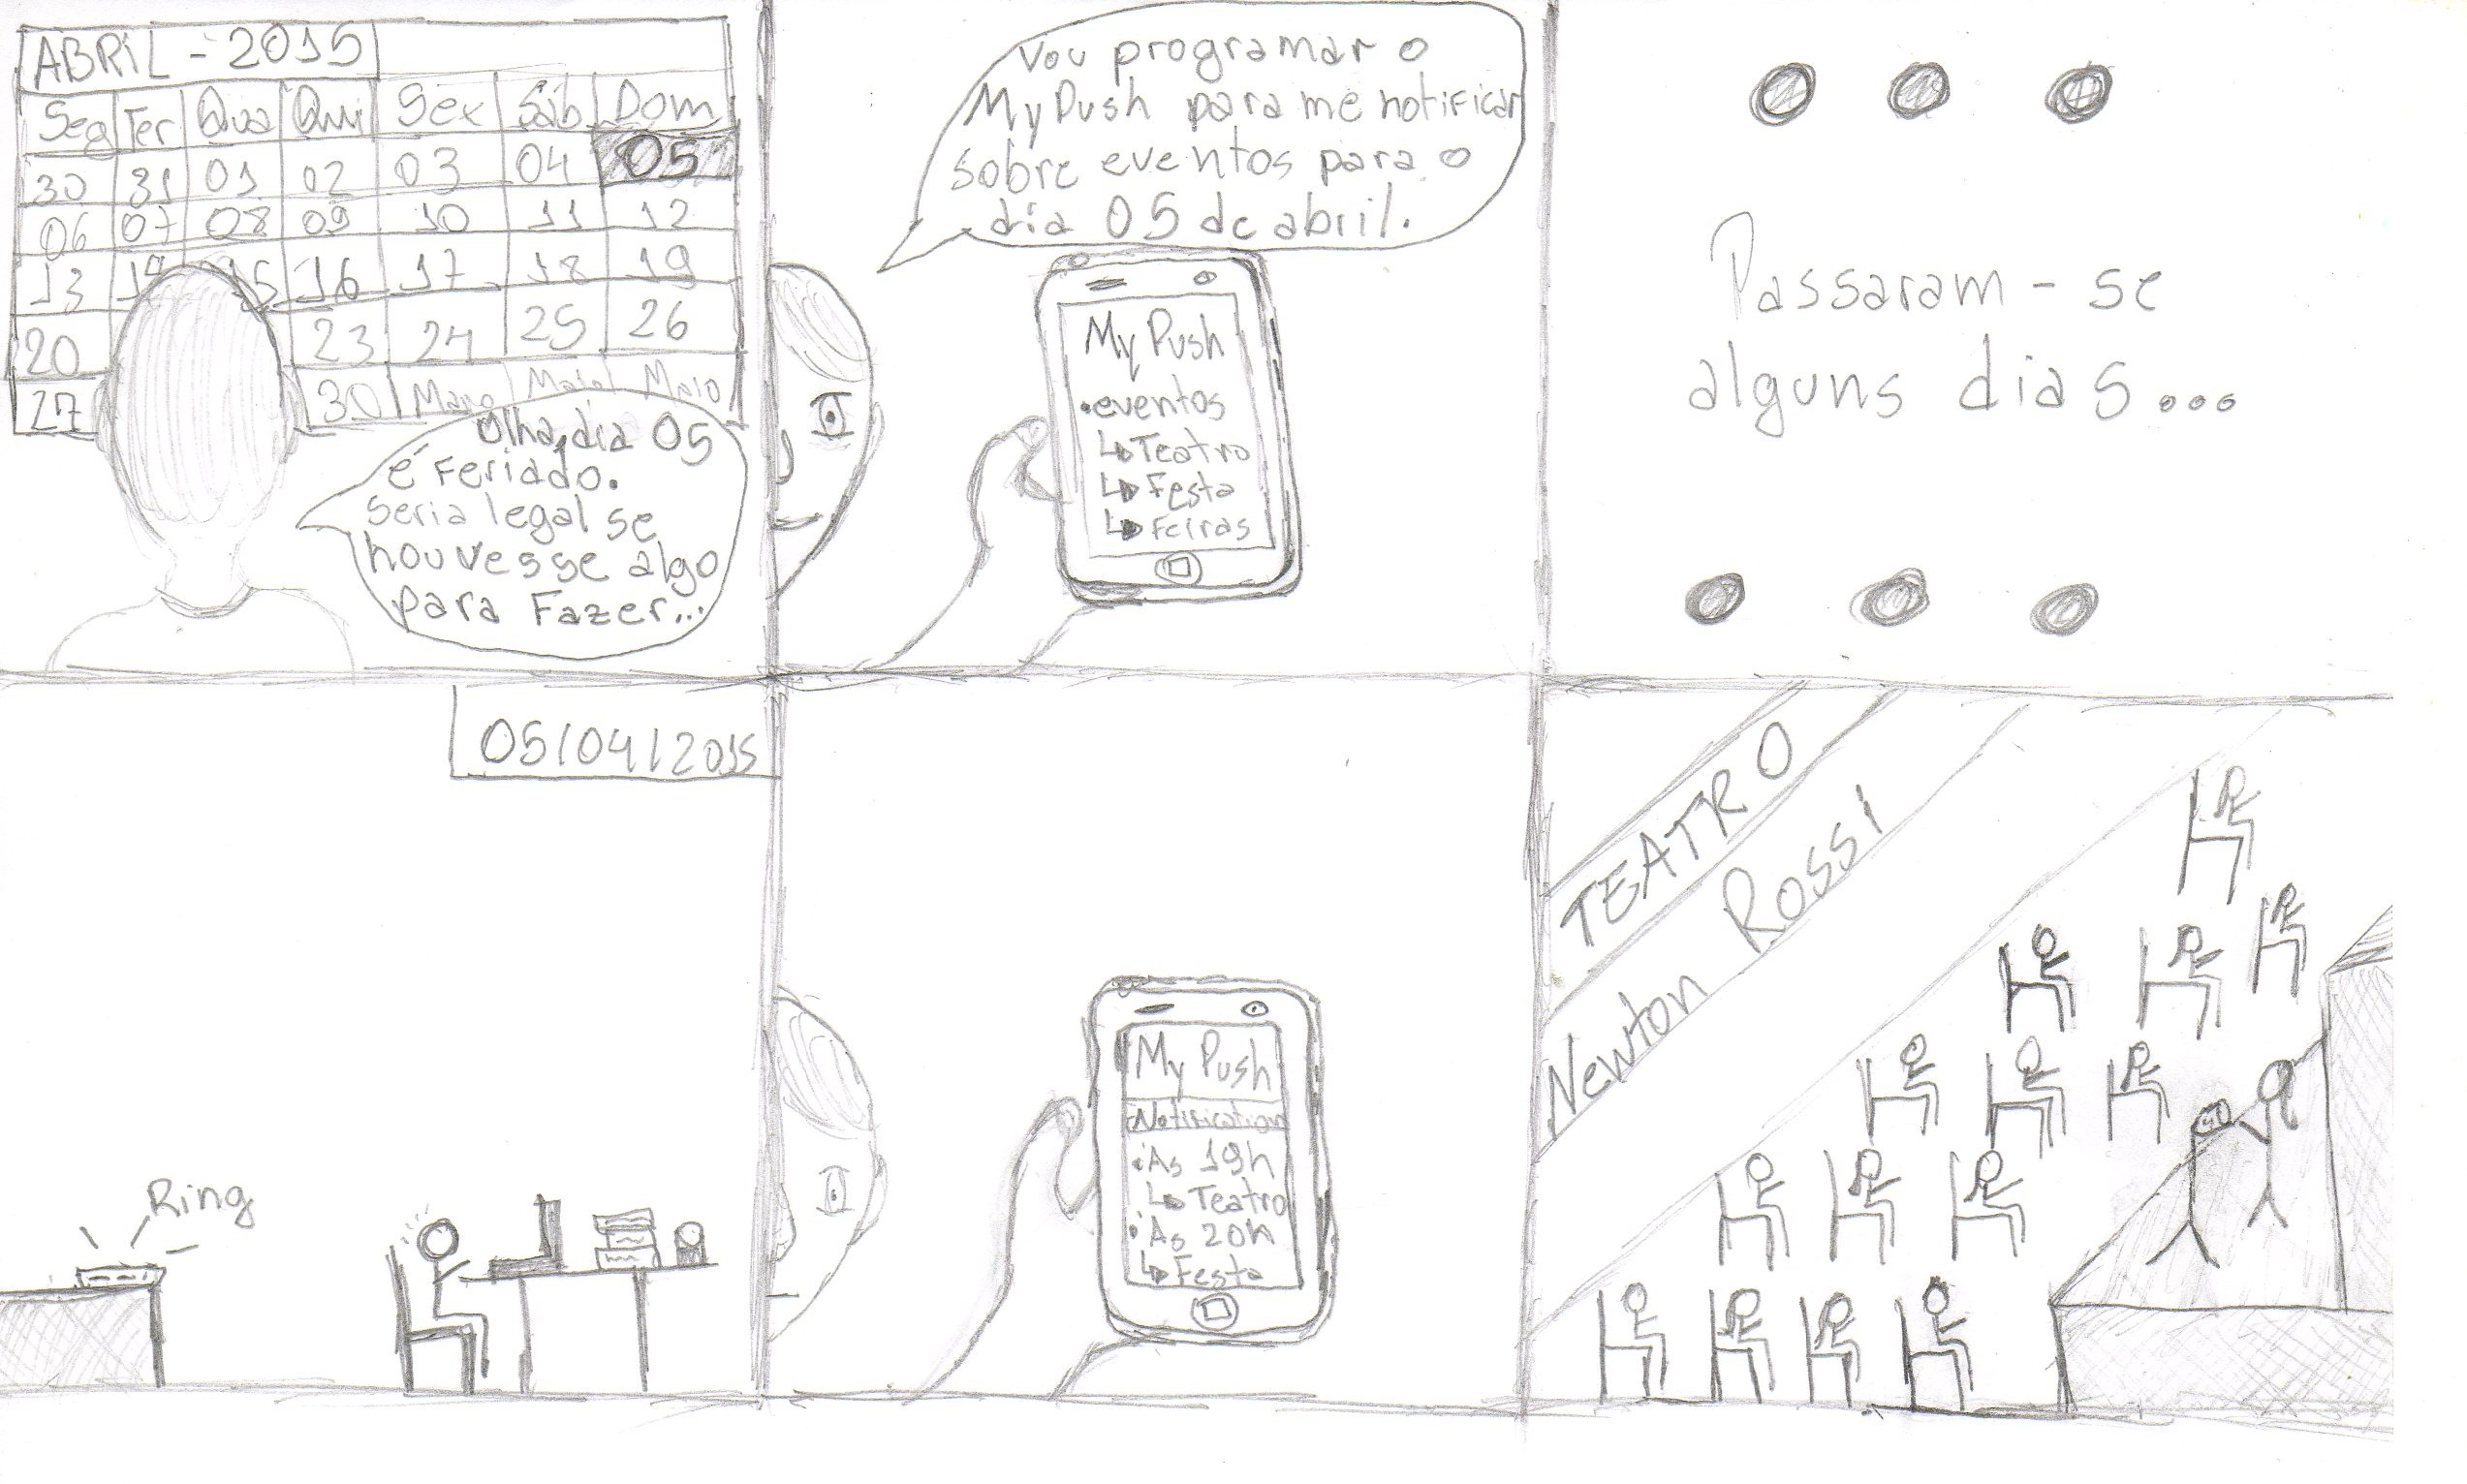
\includegraphics[scale=0.2]{editaveis/figuras/storyboard_papel}
    \caption{\textit{Storyboard} feito à mão.}
    \label{storyboard_papel}
  \end{figure}

\chapter{\textit{Storyboard} feito com a utilização da ferramenta \textit{Bitstrips}.}

 \begin{figure}[!htbp]
    \centering
    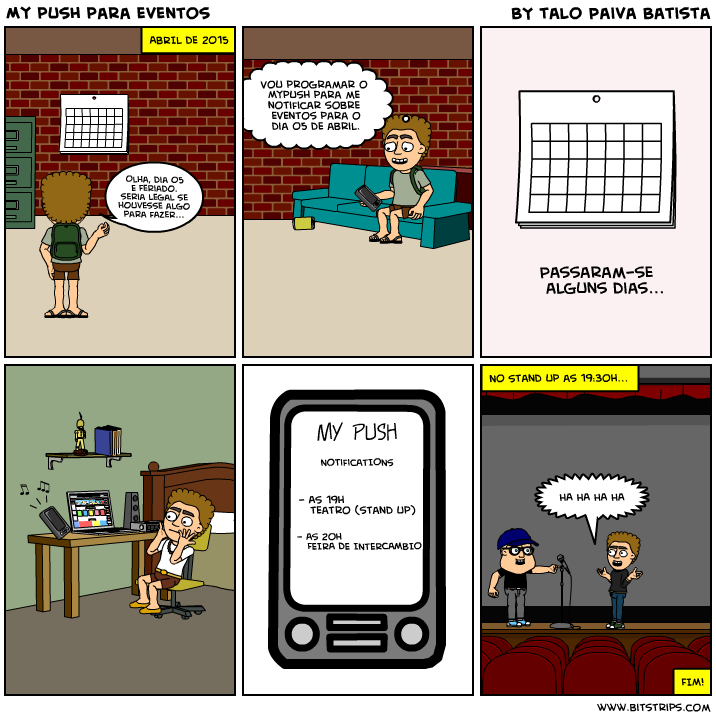
\includegraphics[scale=0.5]{editaveis/figuras/storyboard_ferramenta}
    \caption{\textit{Storyboard} feito com a utilização da ferramenta \textit{Bitstrips}.}
    \label{storyboard_ferramenta}
  \end{figure}

\chapter{Protótipo de papel - Versão 1.0}

  \section*{Protótipo de papel que ilustra a página inicial do sistema.}
  
    \begin{figure}[!htbp]
      \centering
      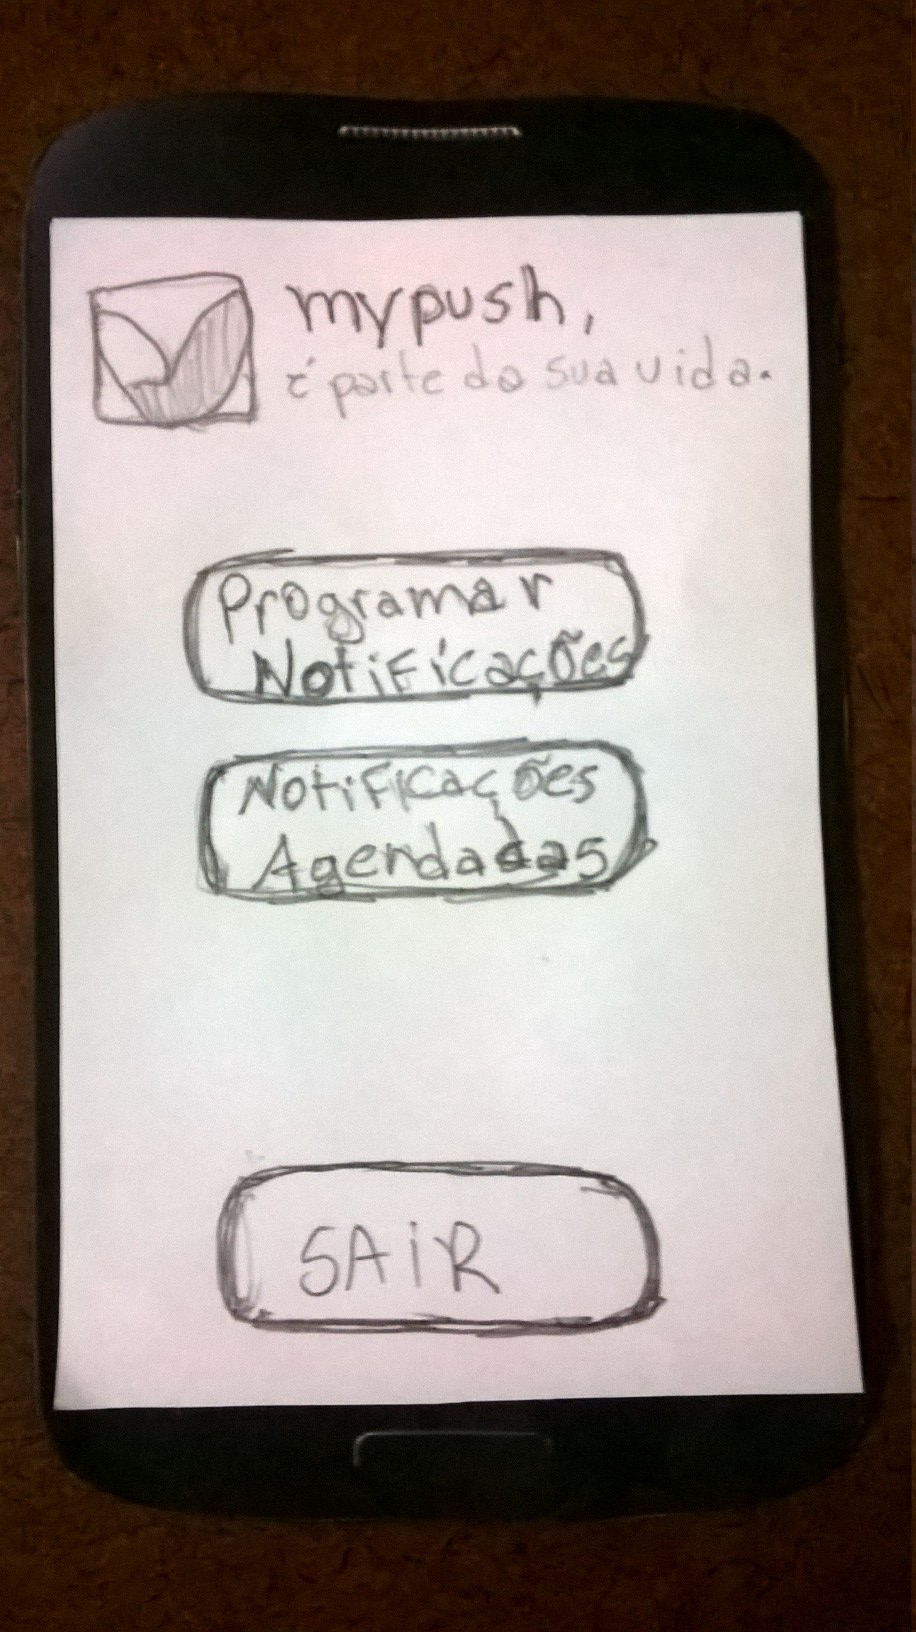
\includegraphics[scale=0.3]{editaveis/figuras/prototipo_papel_v1/pagina_inicial}
      \caption{Protótipo de papel que ilustra a página inicial do sistema.}
      \label{pagina_inicial_v1}
    \end{figure}
  
    \pagebreak
    \section*{Protótipo de papel que ilustra a funcionalidade procurar por tema.}
    
      \begin{figure}[!htbp]
	\centering
	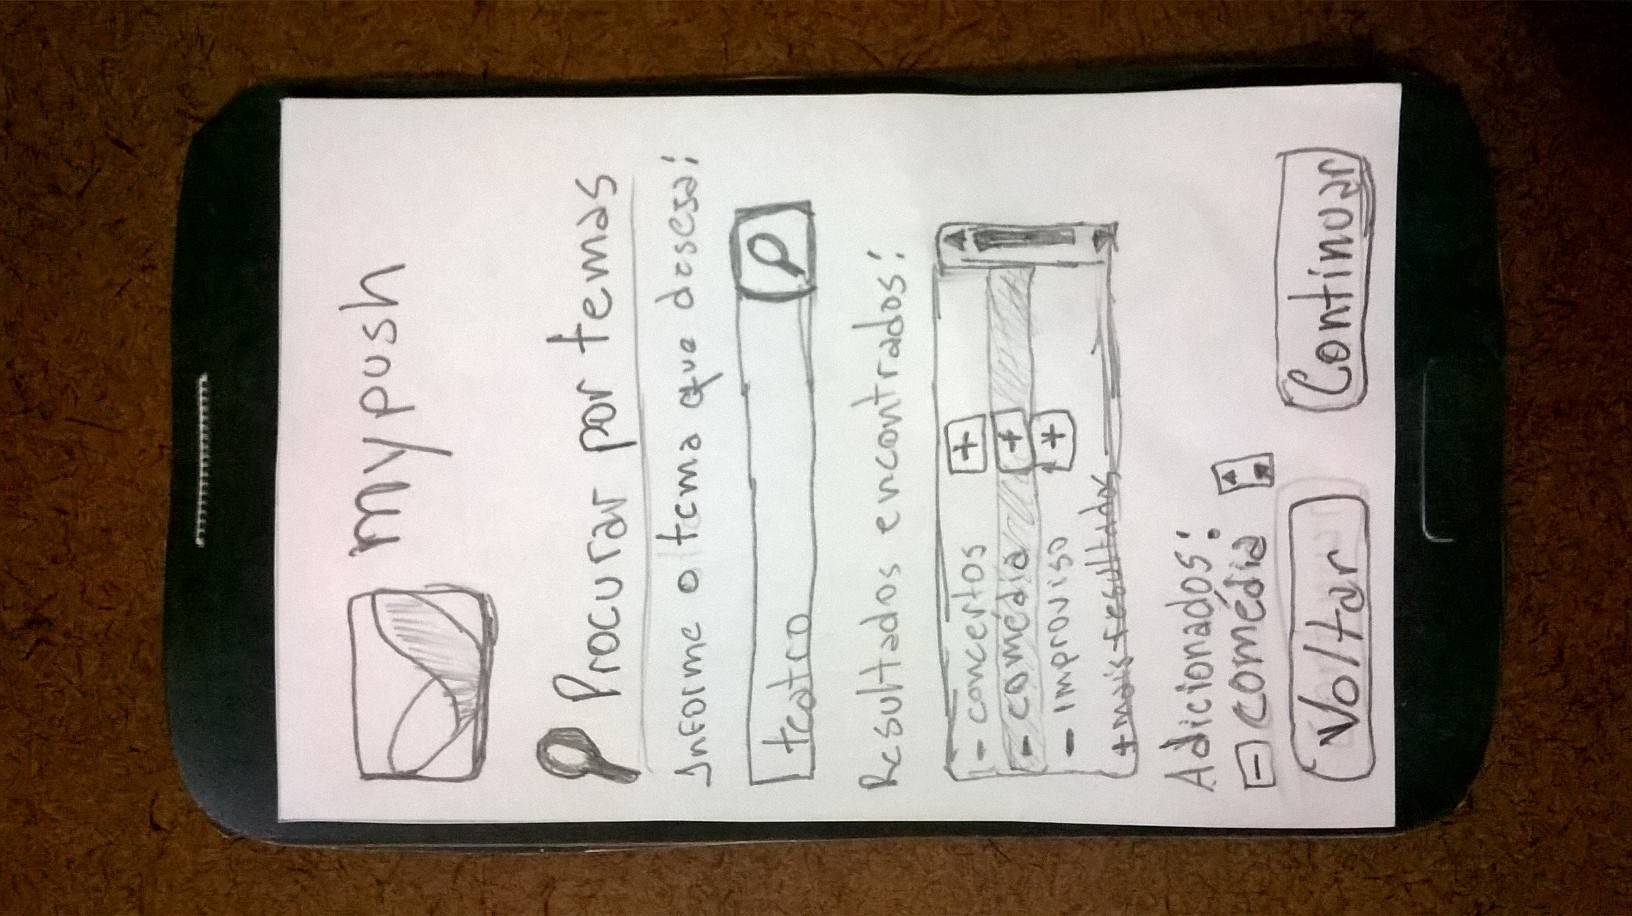
\includegraphics[scale=0.32, angle=-90]{editaveis/figuras/prototipo_papel_v1/procurar_por_temas}
	\caption{Protótipo de papel que ilustra a funcionalidade procurar por tema.}
	\label{procurar_por_temas_v1}
      \end{figure}
    
    \pagebreak
    \section*{Protótipo de papel que ilustra a funcionalidade procurar por tema quando um tema é adicionado.}
    
      \begin{figure}[!htbp]
	\centering
	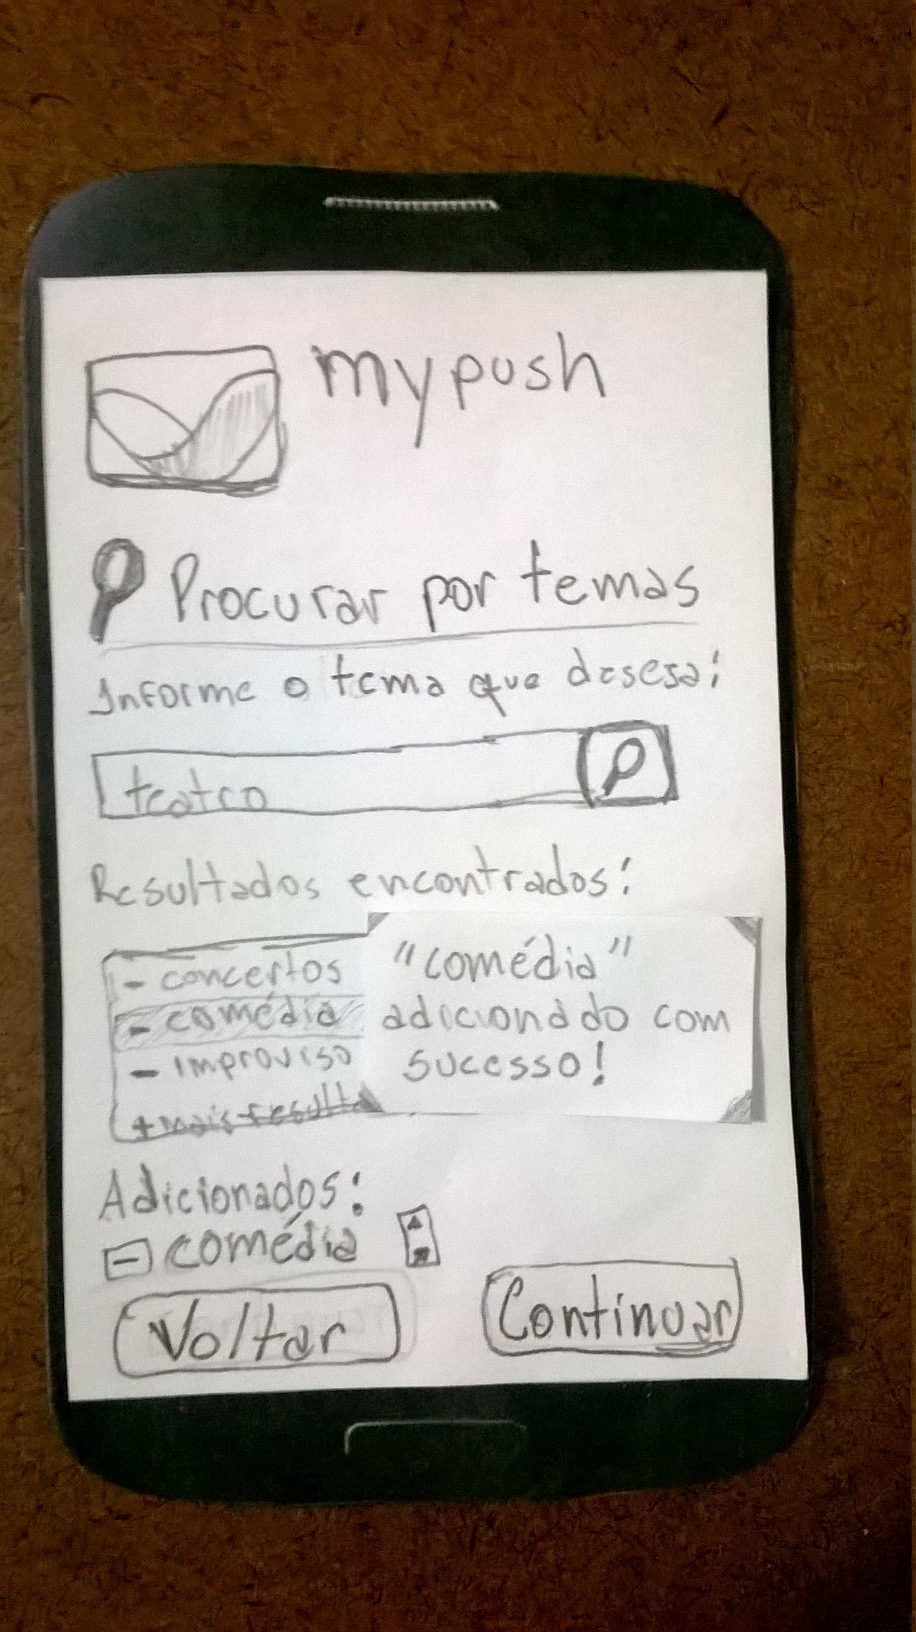
\includegraphics[scale=0.32]{editaveis/figuras/prototipo_papel_v1/tema_adicionado}
	\caption{Protótipo de papel que ilustra a funcionalidade procurar por tema quando um tema é adicionado.}
	\label{tema_adicionado_v1}
      \end{figure}
	
    \pagebreak
    \section*{Protótipo de papel que ilustra a funcionalidade de escolher a data e hora para a notificação.}
    
      \begin{figure}[!htbp]
	\centering
	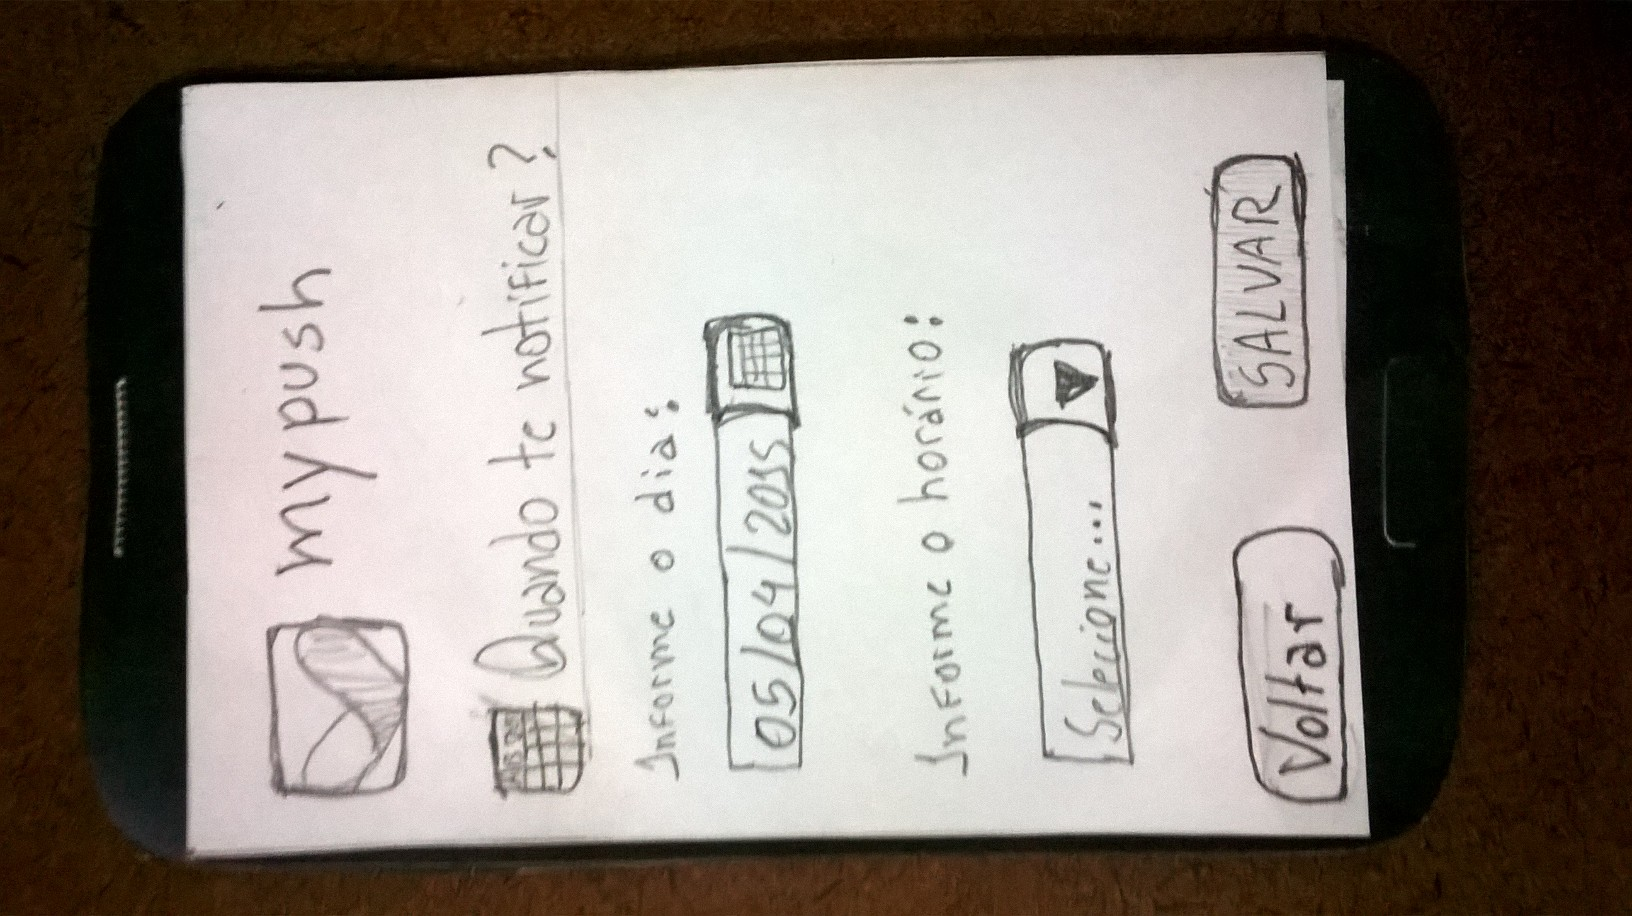
\includegraphics[scale=0.32, angle=-90]{editaveis/figuras/prototipo_papel_v1/quando_notificar}
	\caption{Protótipo de papel que ilustra a funcionalidade de escolher a data e hora para a notificação.}
	\label{quando_notificar_v1}
      \end{figure}
      
    \pagebreak
    \section*{Protótipo de papel que ilustra a funcionalidade de escolher a data por um calendário.}
    
      \begin{figure}[!htbp]
	\centering
	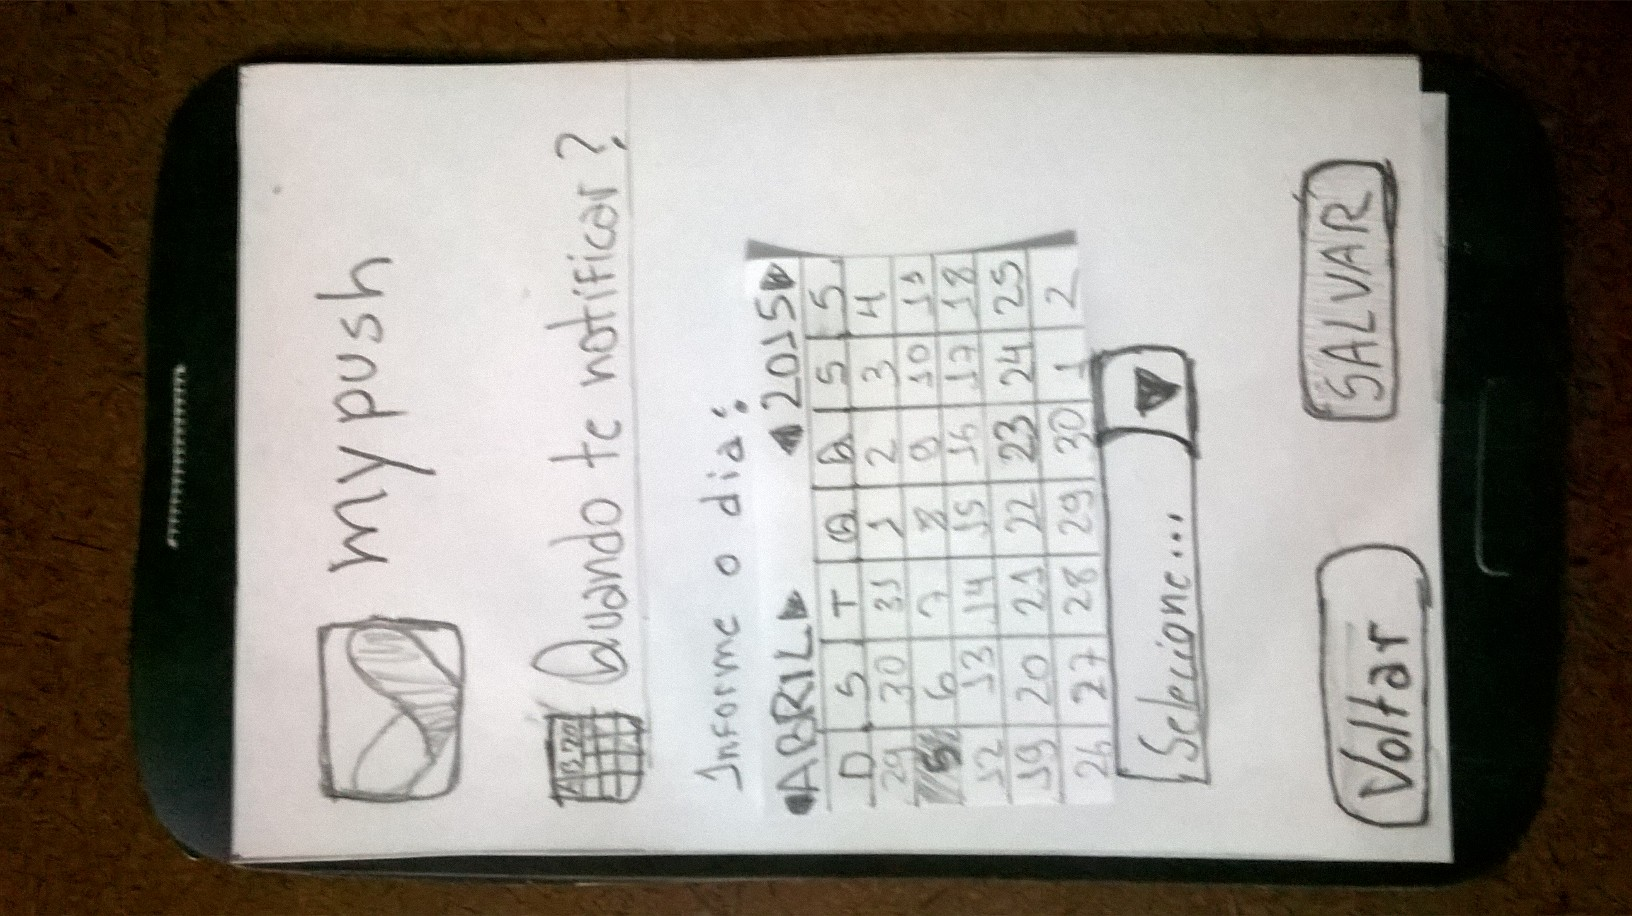
\includegraphics[scale=0.32, angle=-90]{editaveis/figuras/prototipo_papel_v1/quando_notificar_data}
	\caption{Protótipo de papel que ilustra a funcionalidade de escolher a data por um calendário.}
	\label{quando_notificar_data_v1}
      \end{figure}
    
    \pagebreak
    \section*{Protótipo de papel que ilustra a funcionalidade de escolher a hora por um \textit{dropdown}.}
    
      \begin{figure}[!htbp]
	\centering
	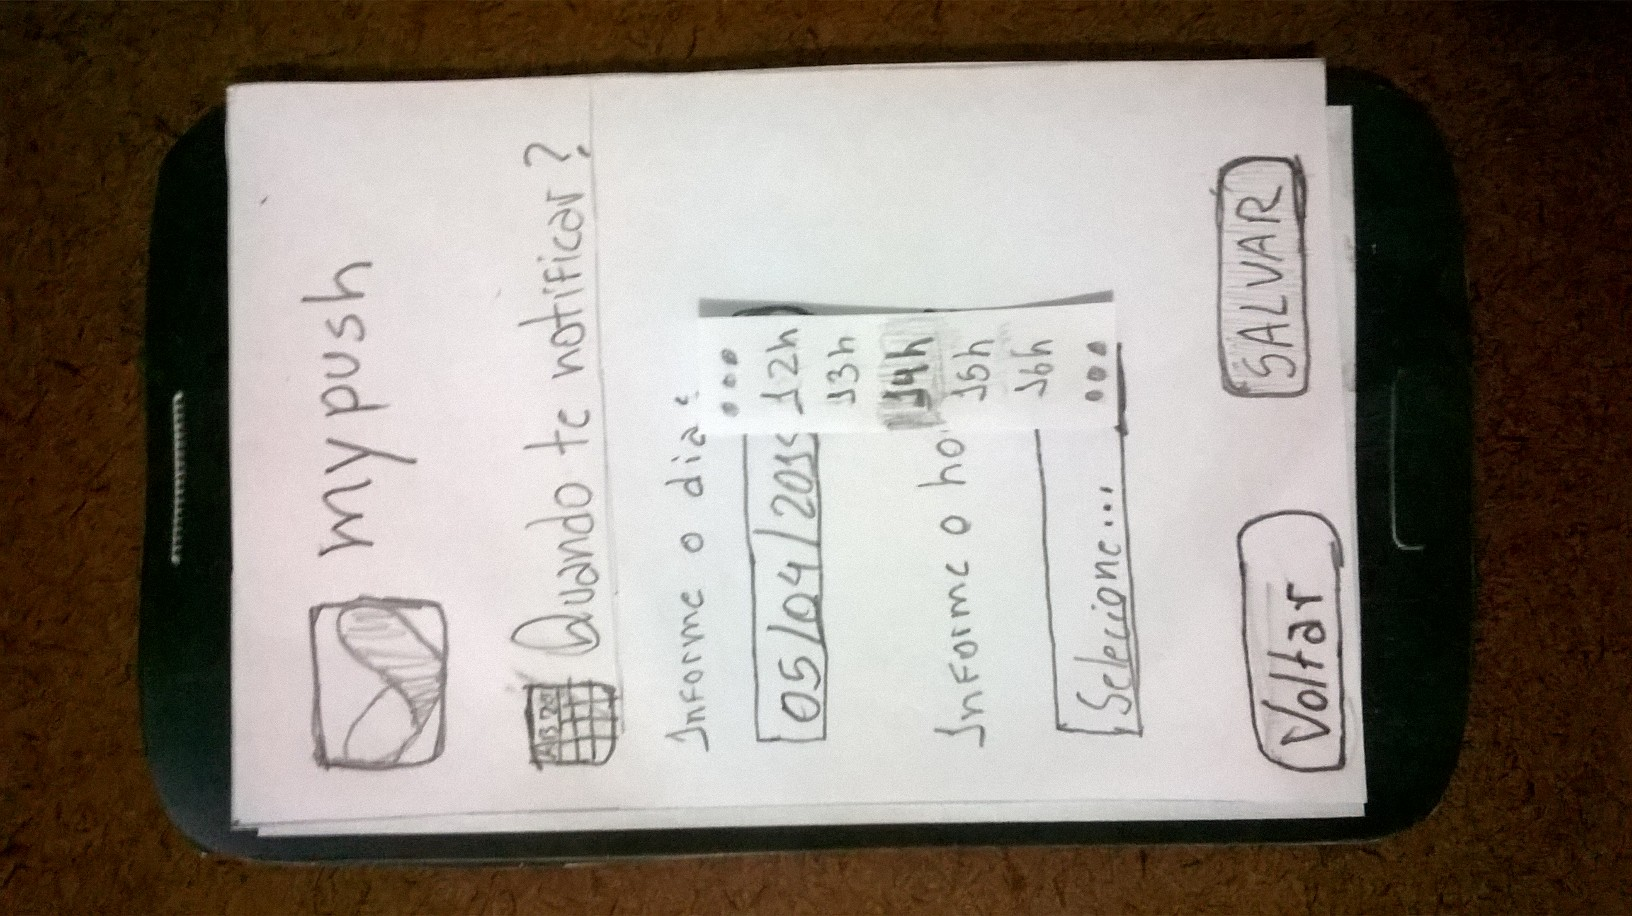
\includegraphics[scale=0.32, angle=-90]{editaveis/figuras/prototipo_papel_v1/quando_notificar_horario}
	\caption{Protótipo de papel que ilustra a funcionalidade de escolher a hora por um \textit{dropdown}.}
	\label{quando_notificar_horario_v1}
      \end{figure}
      
    \pagebreak
    \section*{Protótipo de papel que ilustra a mensagem de notificação salva.}
    
      \begin{figure}[!htbp]
	\centering
	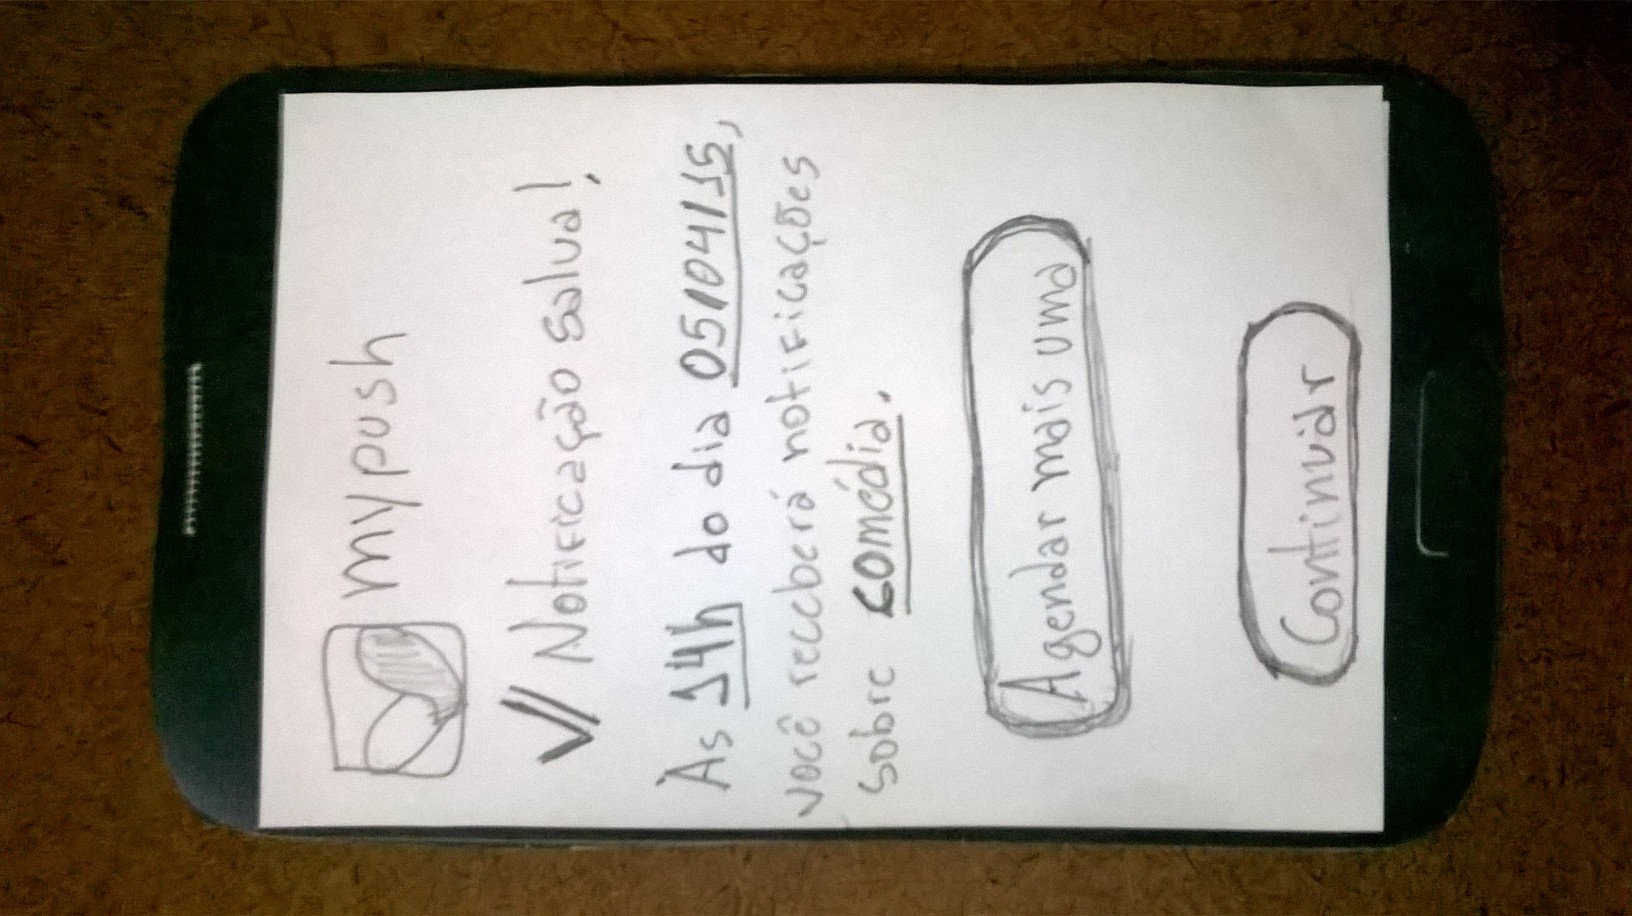
\includegraphics[scale=0.32, angle=-90]{editaveis/figuras/prototipo_papel_v1/notificacao_salva}
	\caption{Protótipo de papel que ilustra a mensagem de notificação salva.}
	\label{notificacao_salva_v1}
      \end{figure}
    
    \pagebreak
    \section*{Protótipo de papel que ilustra a página de notificações agendadas.}
    
      \begin{figure}[!htbp]
	\centering
	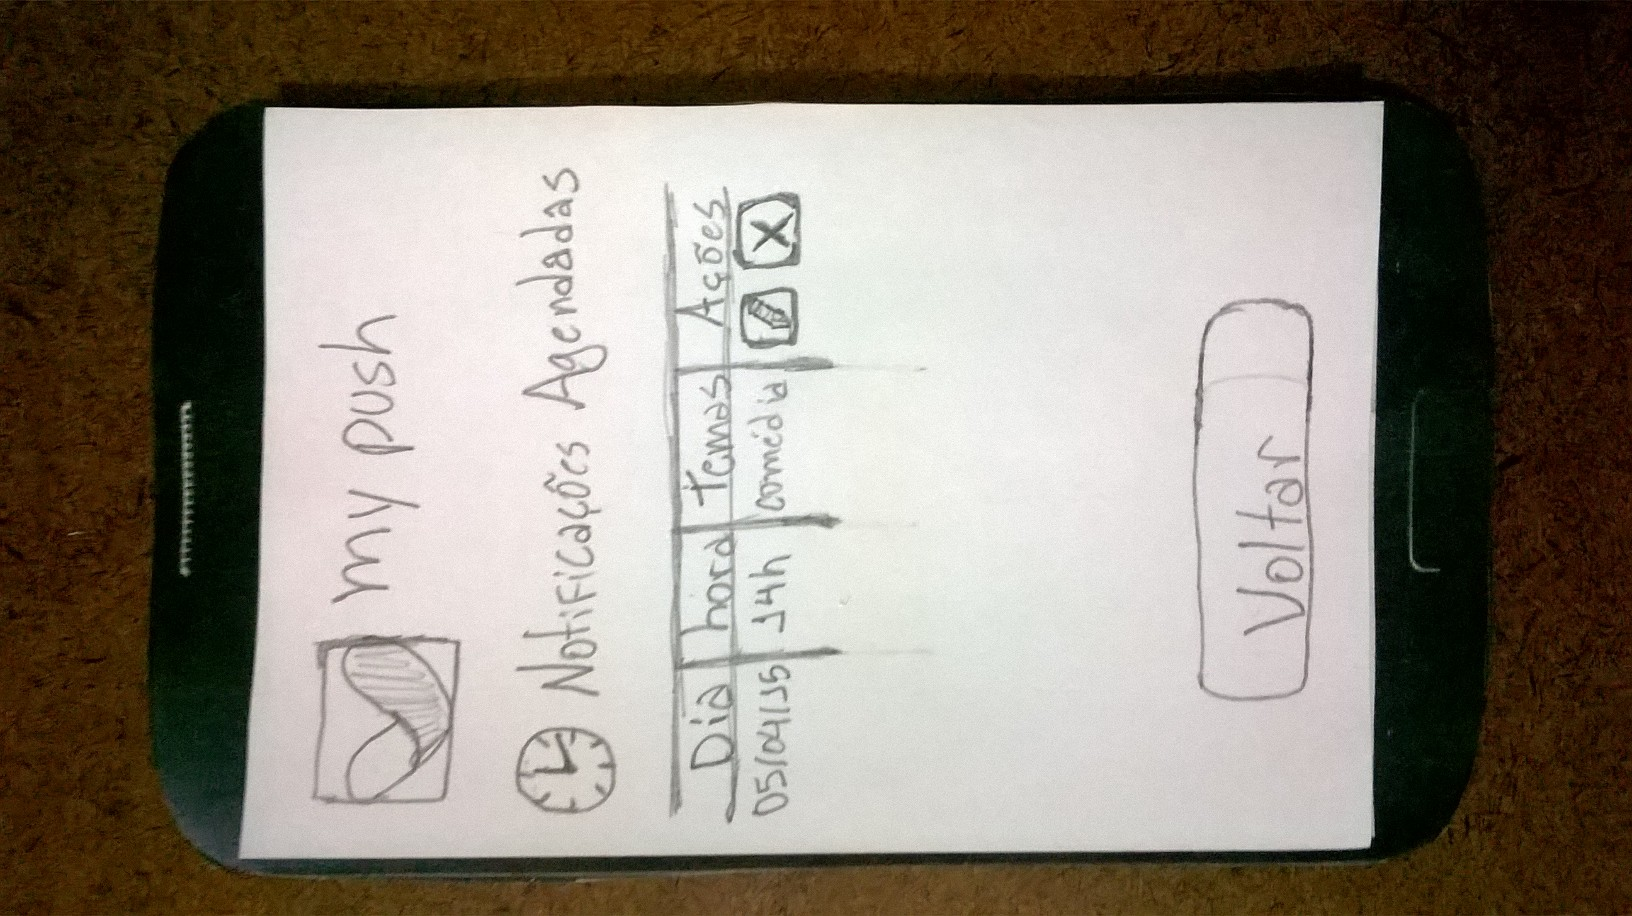
\includegraphics[scale=0.32, angle=-90]{editaveis/figuras/prototipo_papel_v1/notificacoes_agendadas}
	\caption{Protótipo de papel que ilustra a página de notificações agendadas.}
	\label{notificacoes_agendadas_v1}
      \end{figure}
    
    \pagebreak
    \section*{Protótipo de papel que ilustra a mensagem de confirmação de exclusão de notificação.}
    
      \begin{figure}[!htbp]
	\centering
	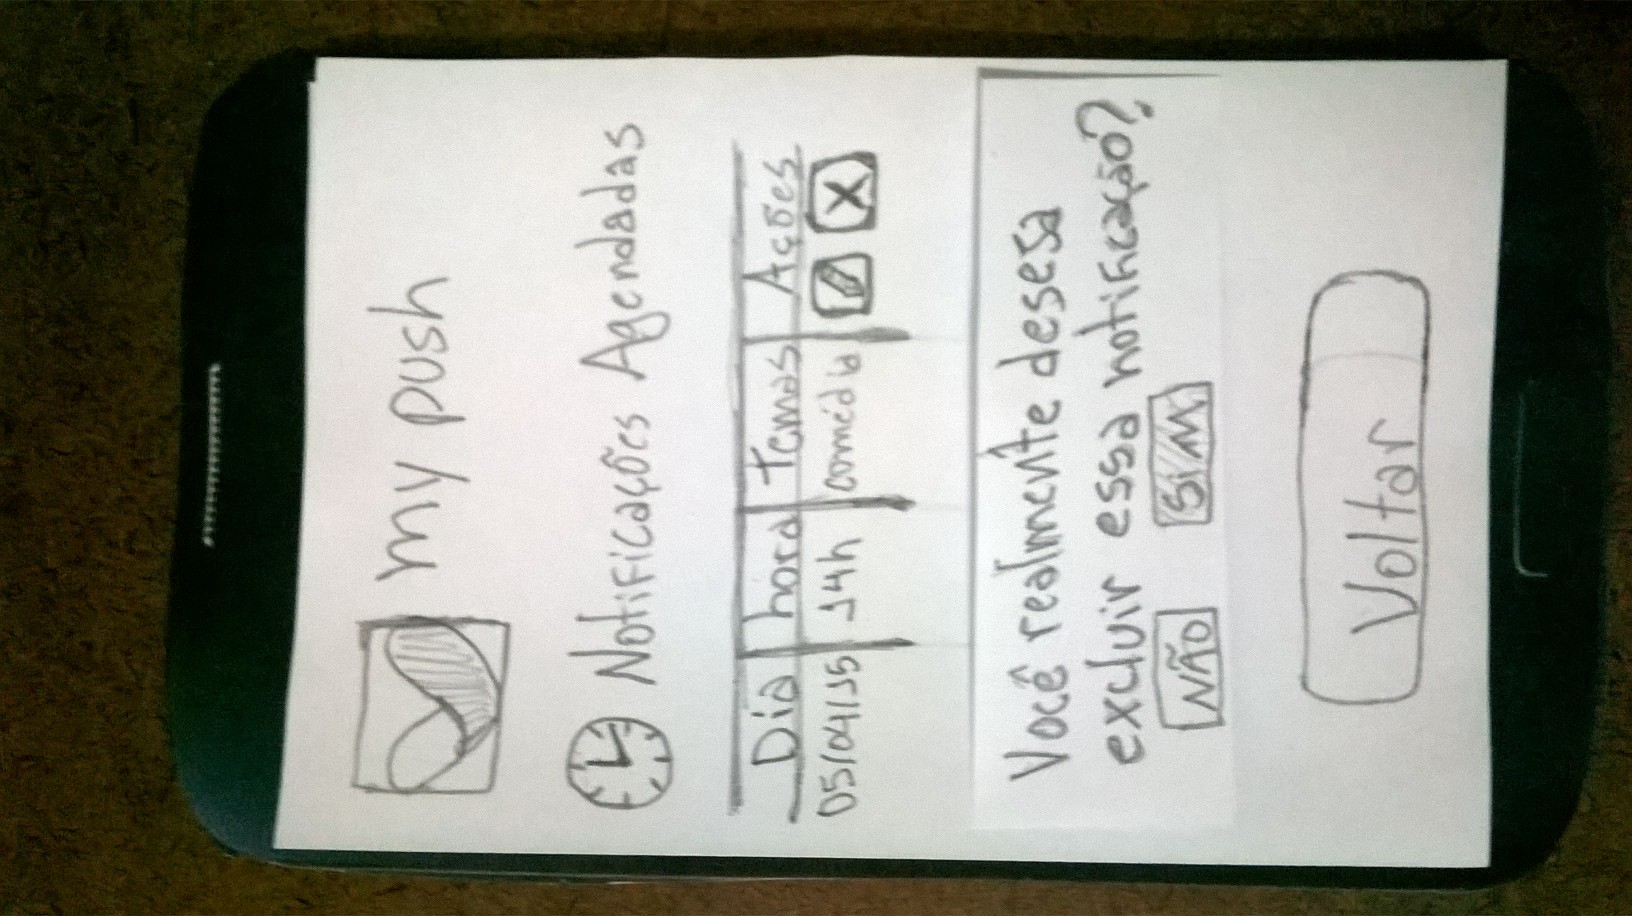
\includegraphics[scale=0.32, angle=-90]{editaveis/figuras/prototipo_papel_v1/confirmacao_excluir_notificacao}
	\caption{Protótipo de papel que ilustra a mensagem de confirmação de exclusão de notificação.}
	\label{confirmacao_excluir_notificacao_v1}
      \end{figure}
    
    \pagebreak
    \section*{Protótipo de papel que ilustra a página para edição de uma notificação.}
    
      \begin{figure}[!htbp]
	\centering
	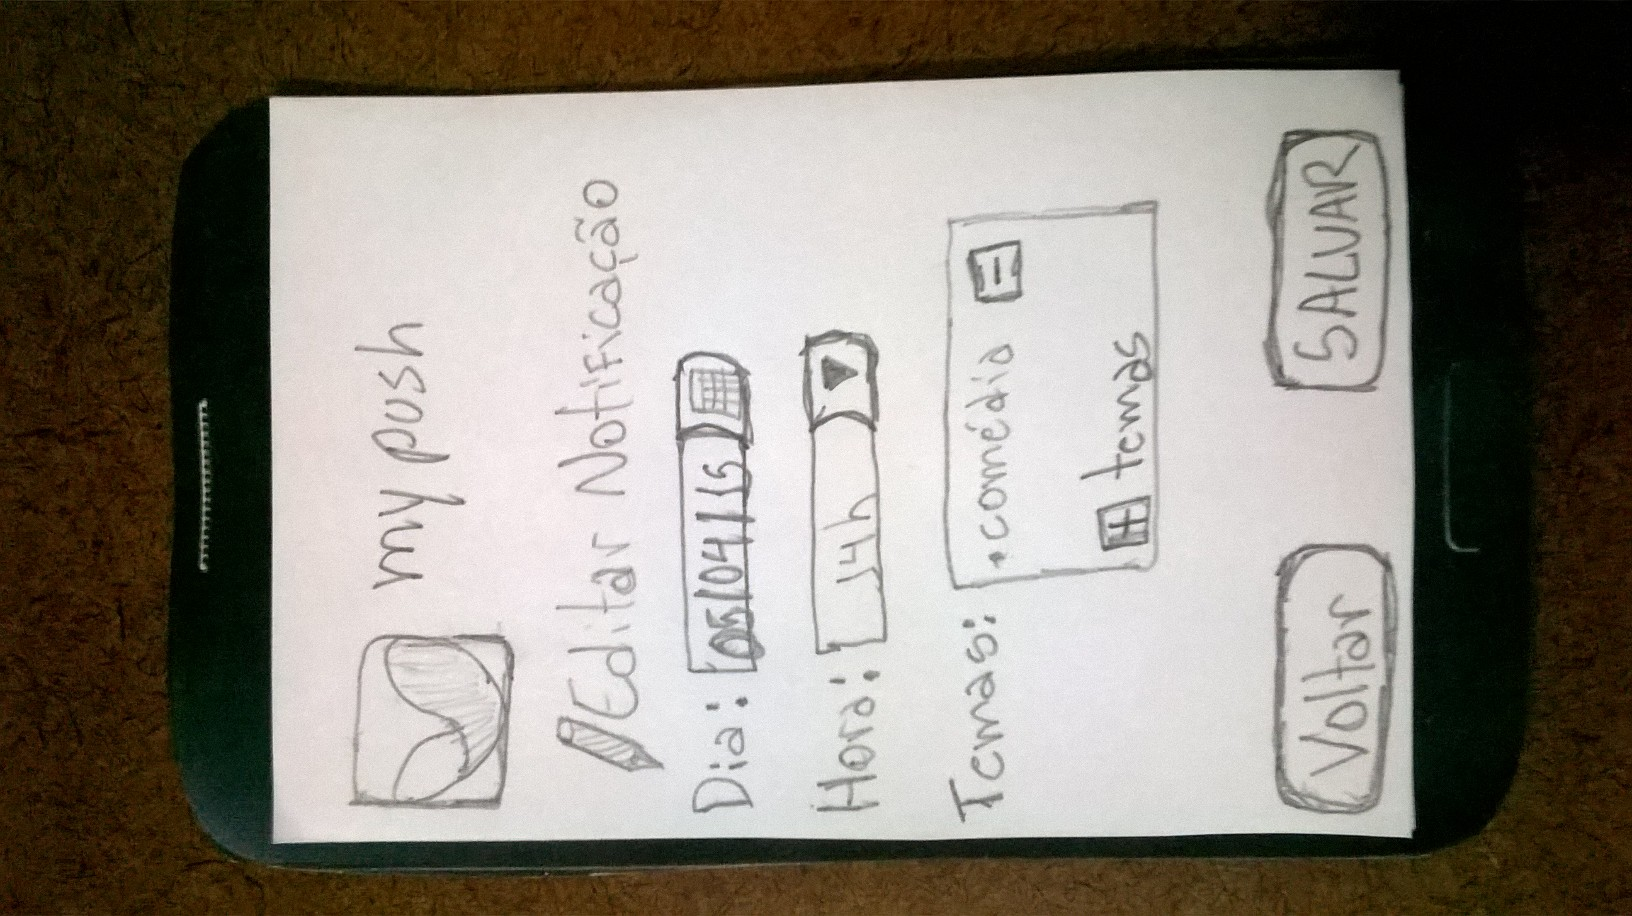
\includegraphics[scale=0.32, angle=-90]{editaveis/figuras/prototipo_papel_v1/editar_notificacao}
	\caption{Protótipo de papel que ilustra a página para edição de uma notificação.}
	\label{editar_notificacao_v1}
      \end{figure}
    
    \pagebreak
    \section*{Protótipo de papel que ilustra um exemplo de notificação no celular.}
    
      \begin{figure}[!htbp]
	\centering
	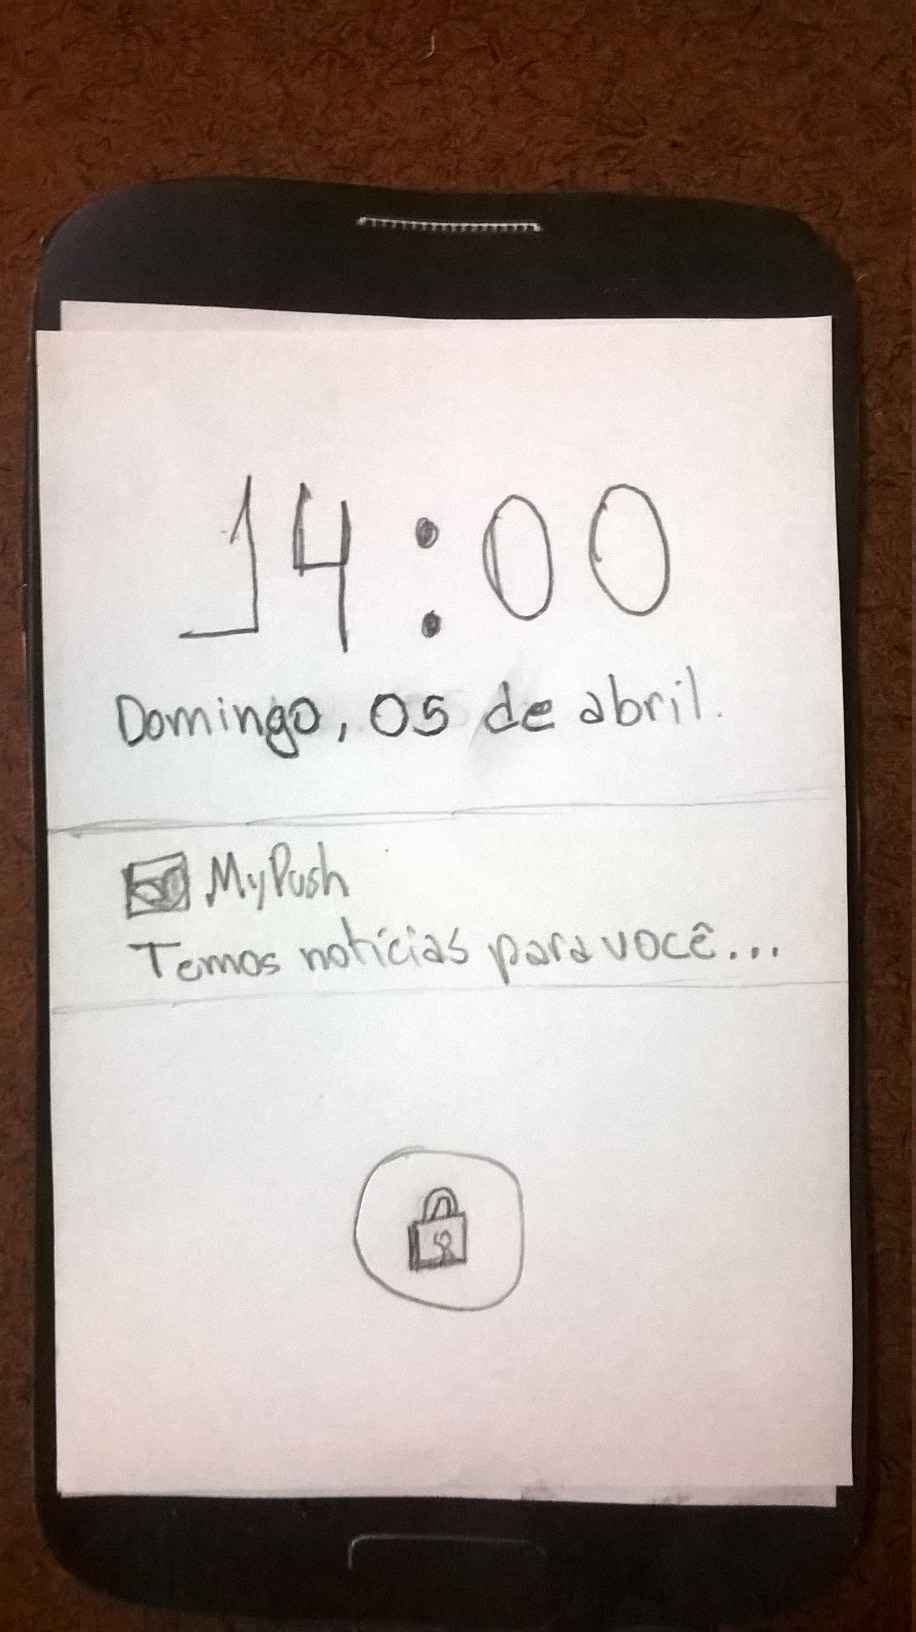
\includegraphics[scale=0.32]{editaveis/figuras/prototipo_papel_v1/tela_bloqueio_notificacao}
	\caption{Protótipo de papel que ilustra um exemplo de notificação no celular.}
	\label{tela_bloqueio_notificacao_v1}
      \end{figure}
    
\chapter{Protótipo de papel - Versão 2.0}
  
  \section*{Protótipo da página inicial com as notificações agendadas}
  
    \begin{figure}[!htbp]
      \centering
      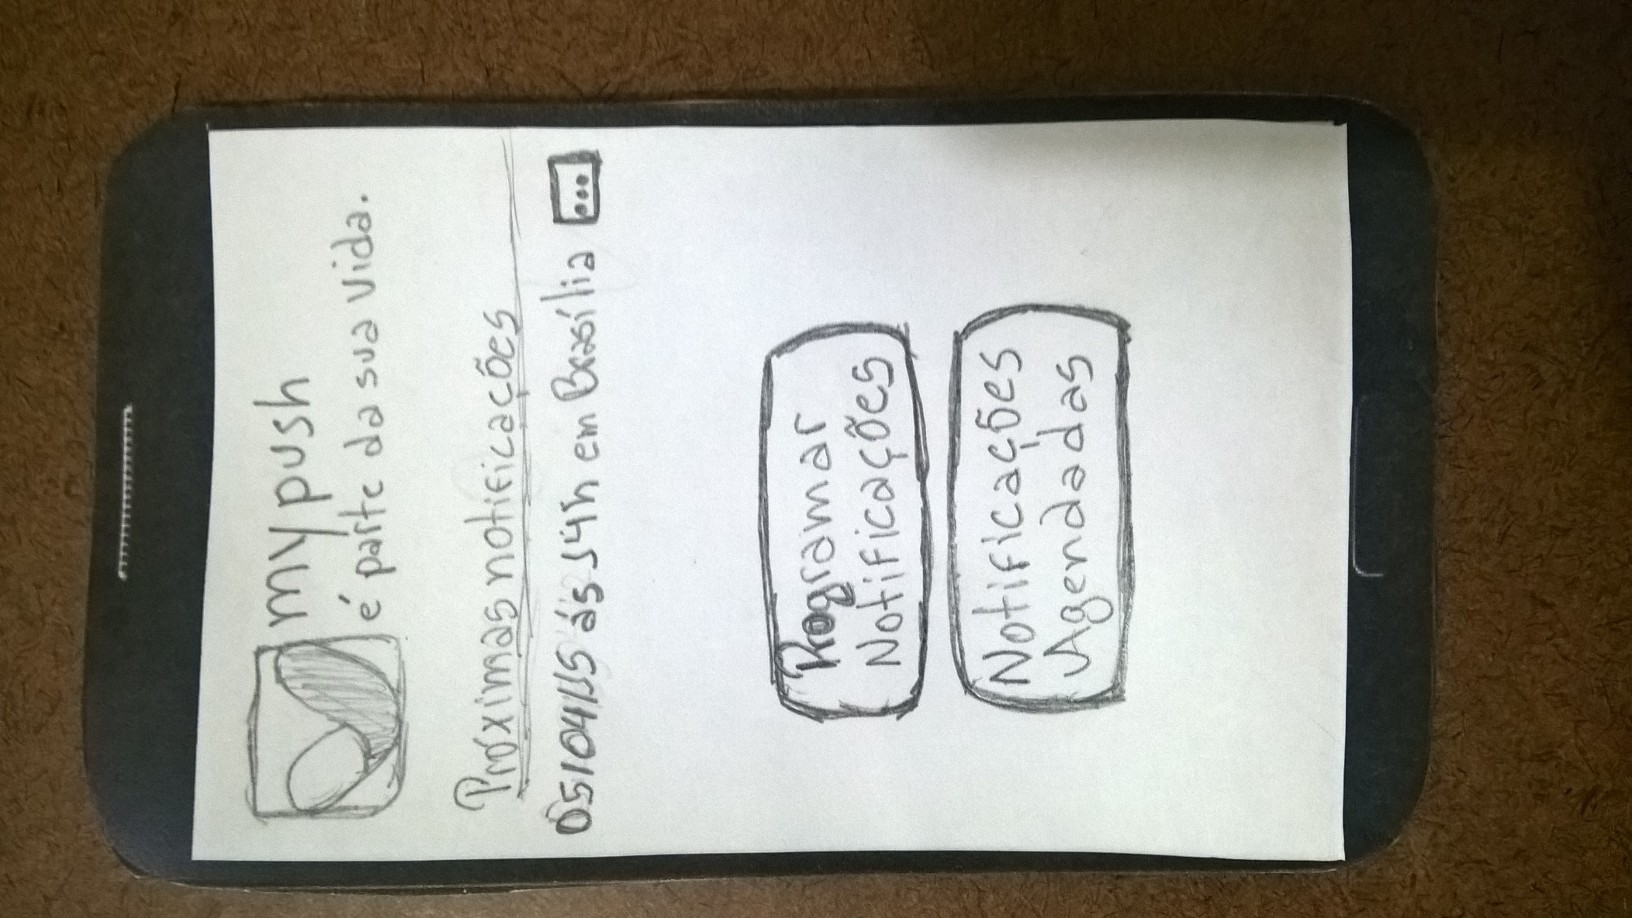
\includegraphics[scale=0.32, angle=-90]{editaveis/figuras/prototipo_papel_v2/pagina_inicial}
      \caption{Protótipo da página inicial com as notificações agendadas}
      \label{pagina_inicial_v2}
    \end{figure}
  
  \pagebreak
  \section*{Protótipo que ilustra a alteração na página de procurar por temas}
    
    \begin{figure}[!htbp]
      \centering
      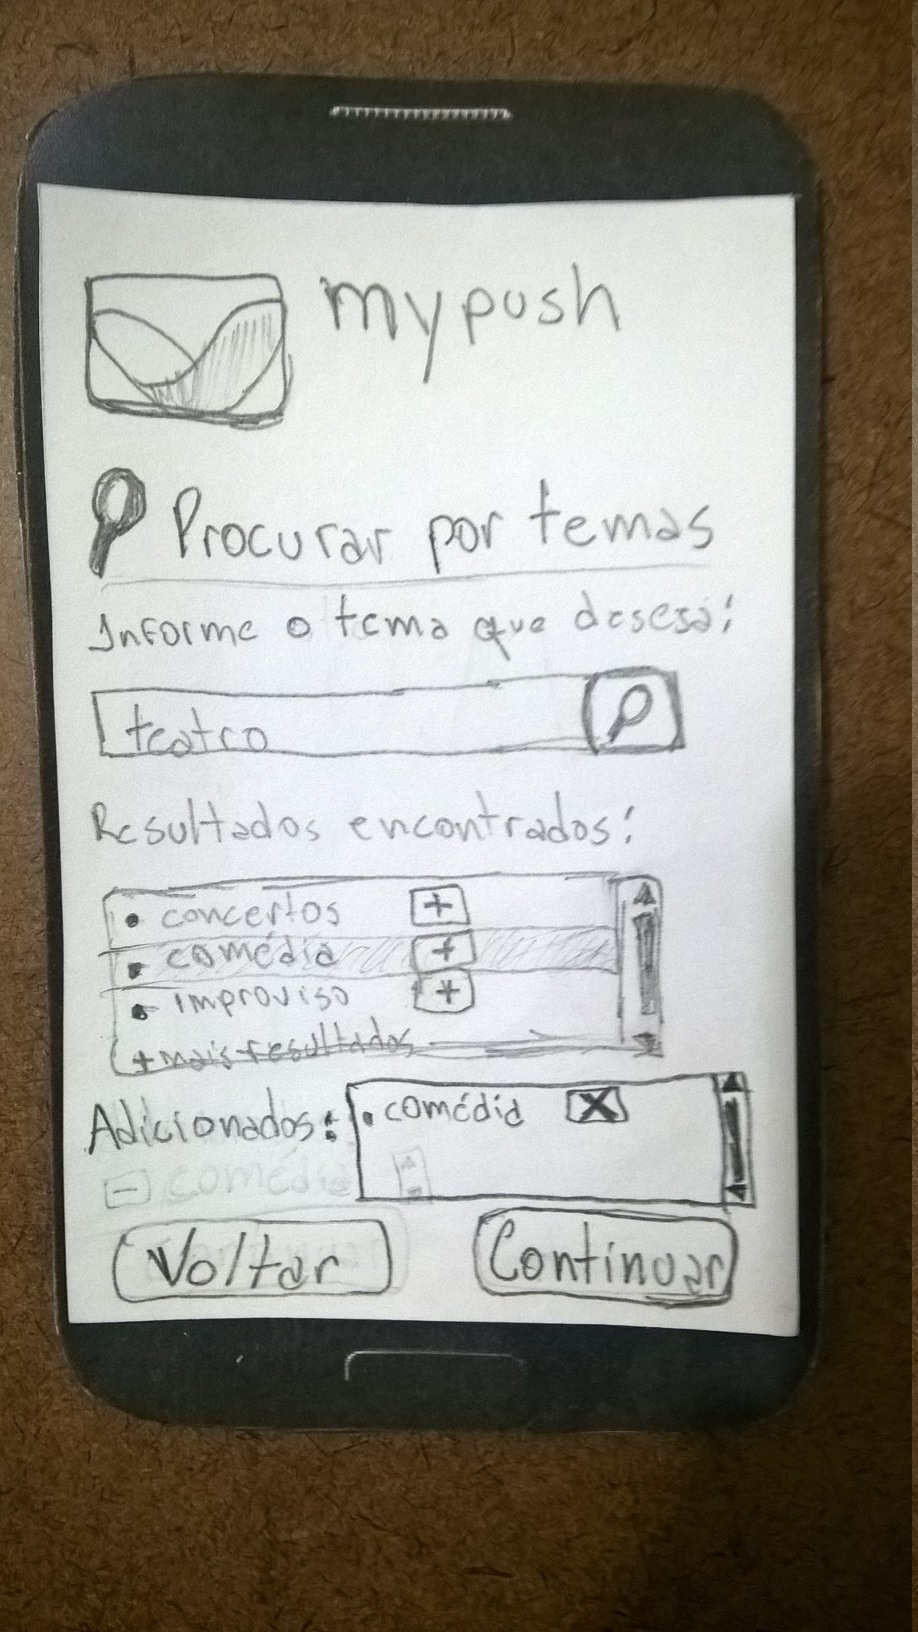
\includegraphics[scale=0.32]{editaveis/figuras/prototipo_papel_v2/procurar_temas}
      \caption{Protótipo que ilustra a alteração na página de procurar por temas}
      \label{procurar_por_temas_v2}
    \end{figure}

  \pagebreak
  \section*{Protótipo que ilustra a alteração na página de procurar por temas}

    \begin{figure}[!htbp]
      \centering
      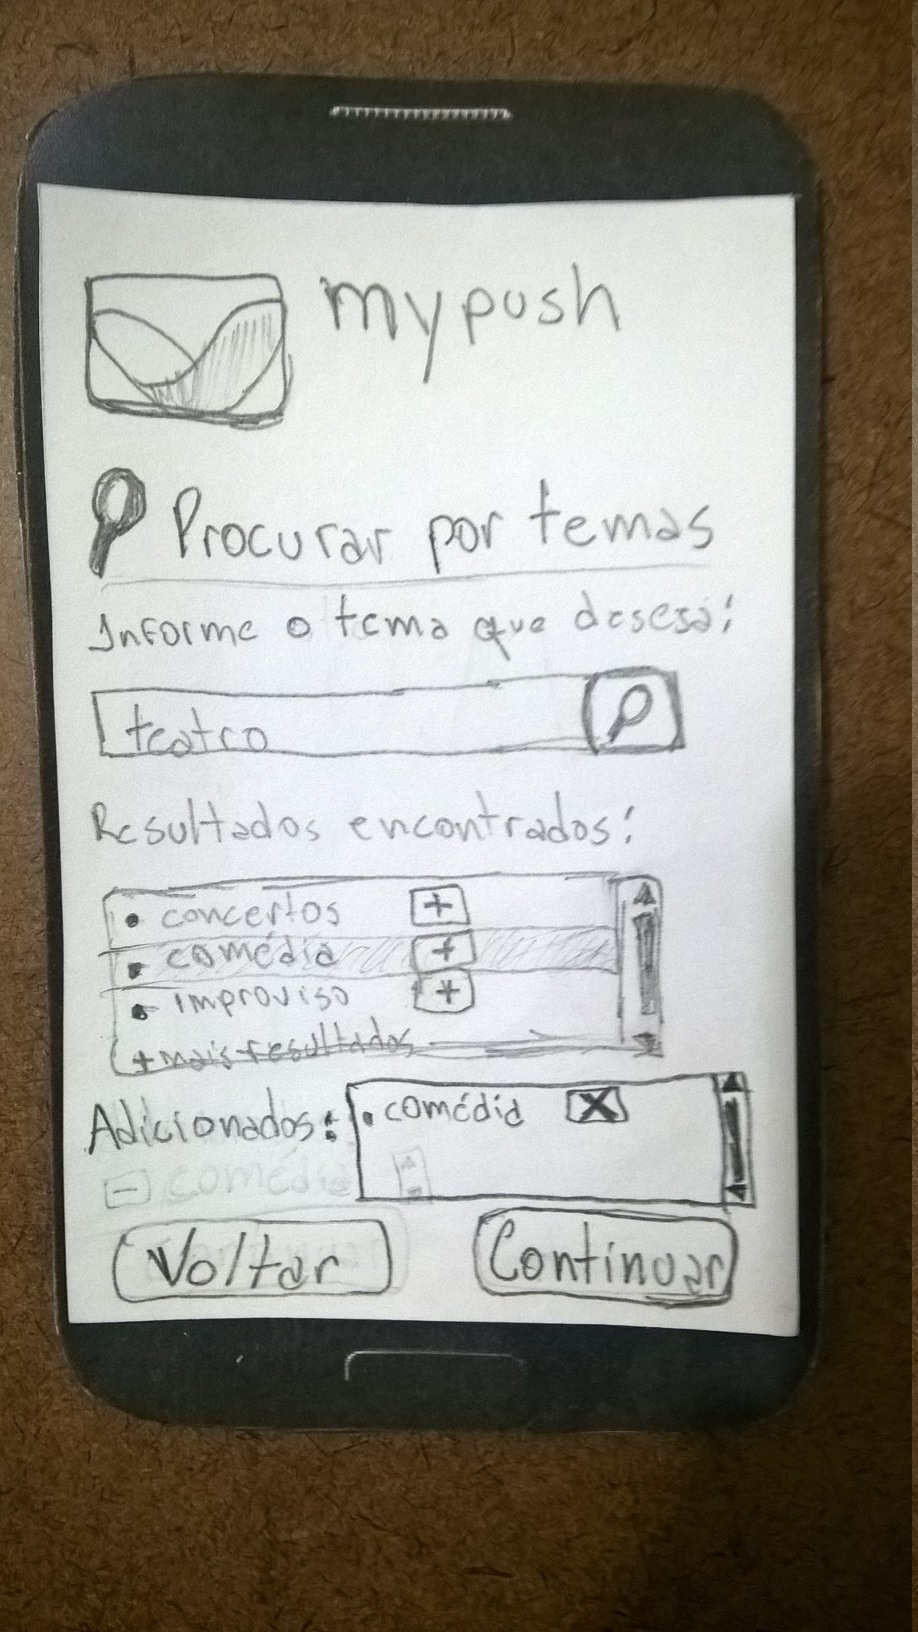
\includegraphics[scale=0.32]{editaveis/figuras/prototipo_papel_v2/procurar_temas}
      \caption{Protótipo que ilustra a alteração na página de procurar por temas}
      \label{procurar_por_temas_v2}
    \end{figure}
   
  \pagebreak
  \section*{Protótipo que ilustra a nova tela de quando notificar}

    \begin{figure}[!htbp]
      \centering
      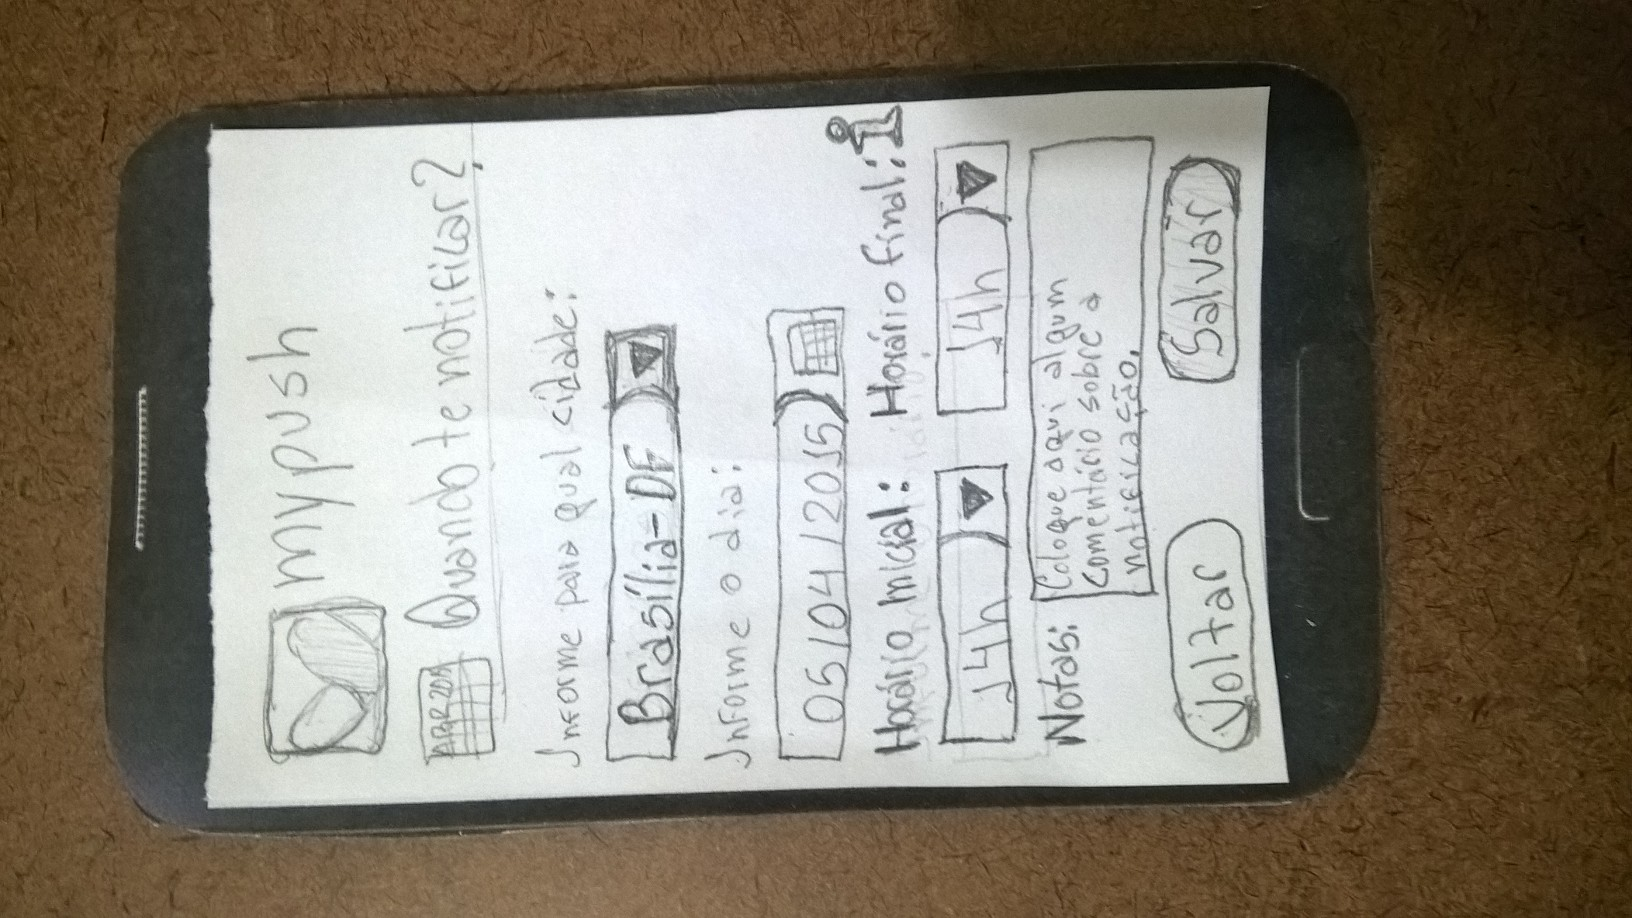
\includegraphics[scale=0.32, angle=-90]{editaveis/figuras/prototipo_papel_v2/quando_notificar}
      \caption{Protótipo que ilustra a alteração na página de quando notificar}
      \label{quando_notificar_v2}
    \end{figure}
  
  \pagebreak
  \section*{Protótipo que ilustra a opção de escolher uma cidade na tela de quando notificar}

    \begin{figure}[!htbp]
      \centering
      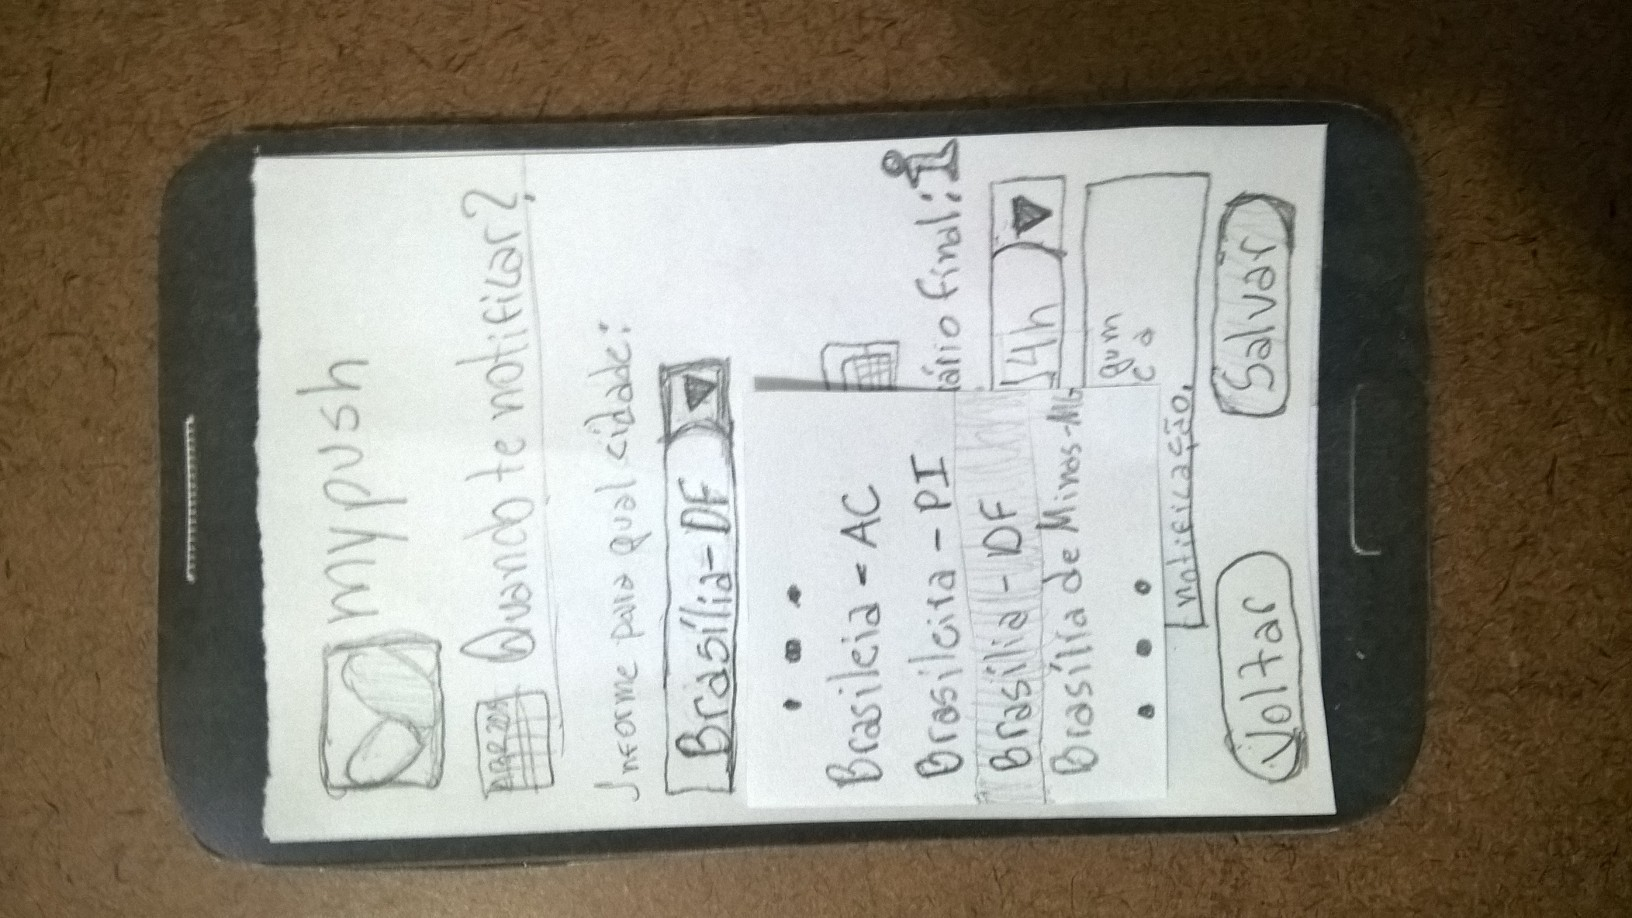
\includegraphics[scale=0.32, angle=-90]{editaveis/figuras/prototipo_papel_v2/quando_notificar_cidade}
      \caption{Protótipo que ilustra a opção de escolher uma cidade na tela de quando notificar}
      \label{quando_notificar_cidade_v2}
    \end{figure}
    
  \pagebreak
  \section*{Protótipo que ilustra a informação sobre o horário}

    \begin{figure}[!htbp]
      \centering
      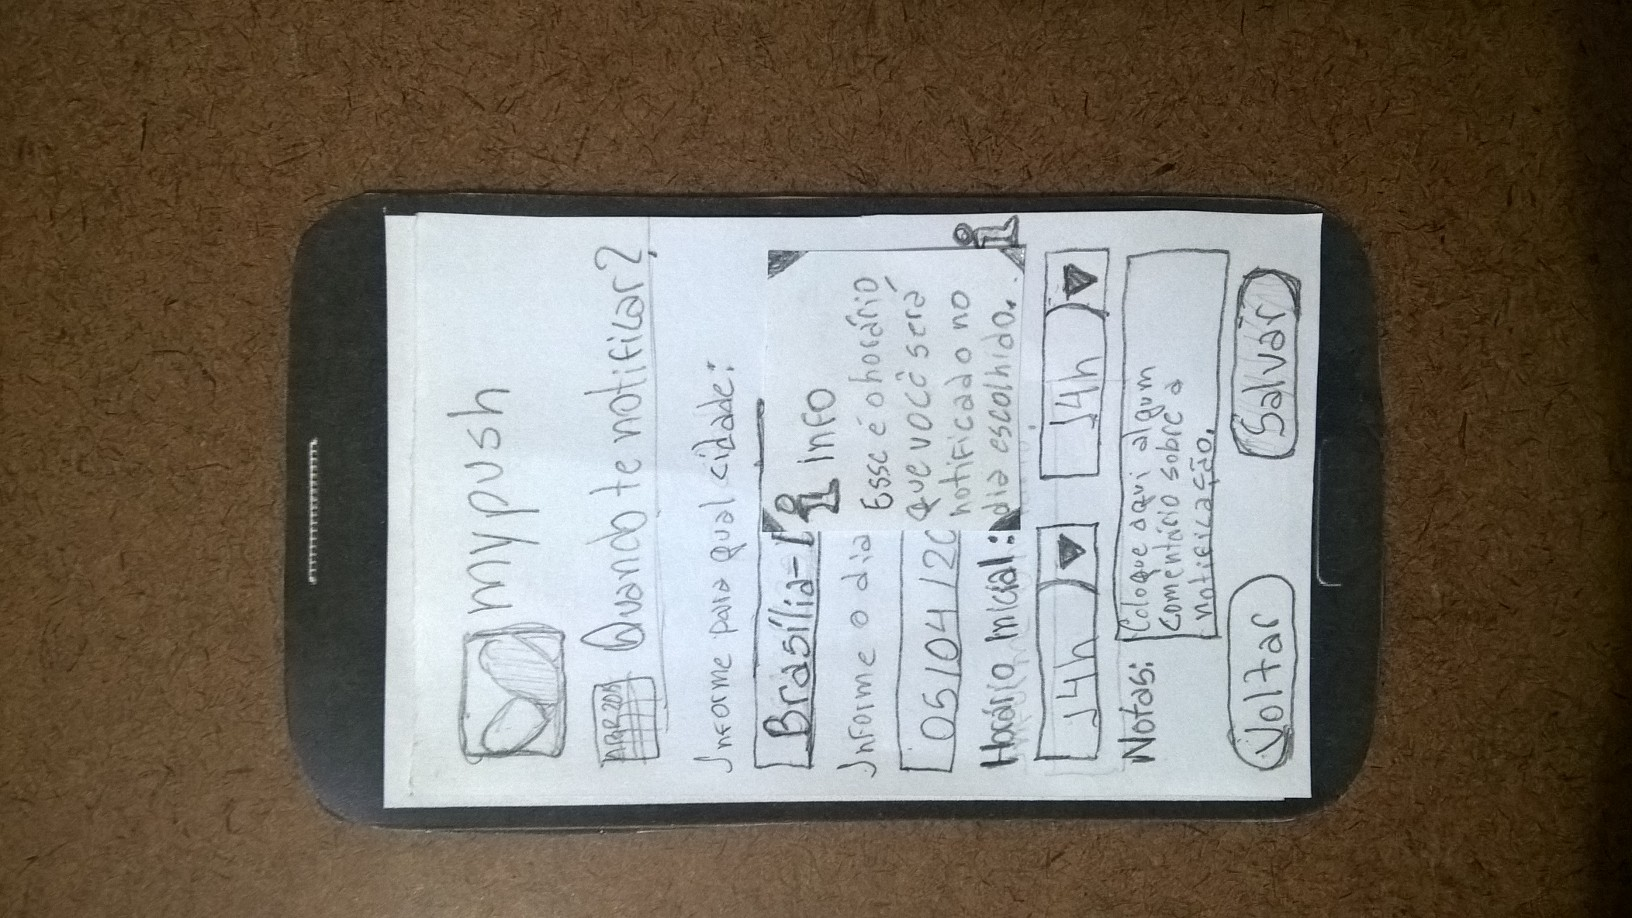
\includegraphics[scale=0.32, angle=-90]{editaveis/figuras/prototipo_papel_v2/quando_notificar_info_horario}
      \caption{Protótipo que ilustra a informação sobre o horário}
      \label{quando_notificar_info_horario_v2}
    \end{figure}
    
  \pagebreak
  \section*{Protótipo que ilustra a mensagem de confirmação para voltar para outra tela}

    \begin{figure}[!htbp]
      \centering
      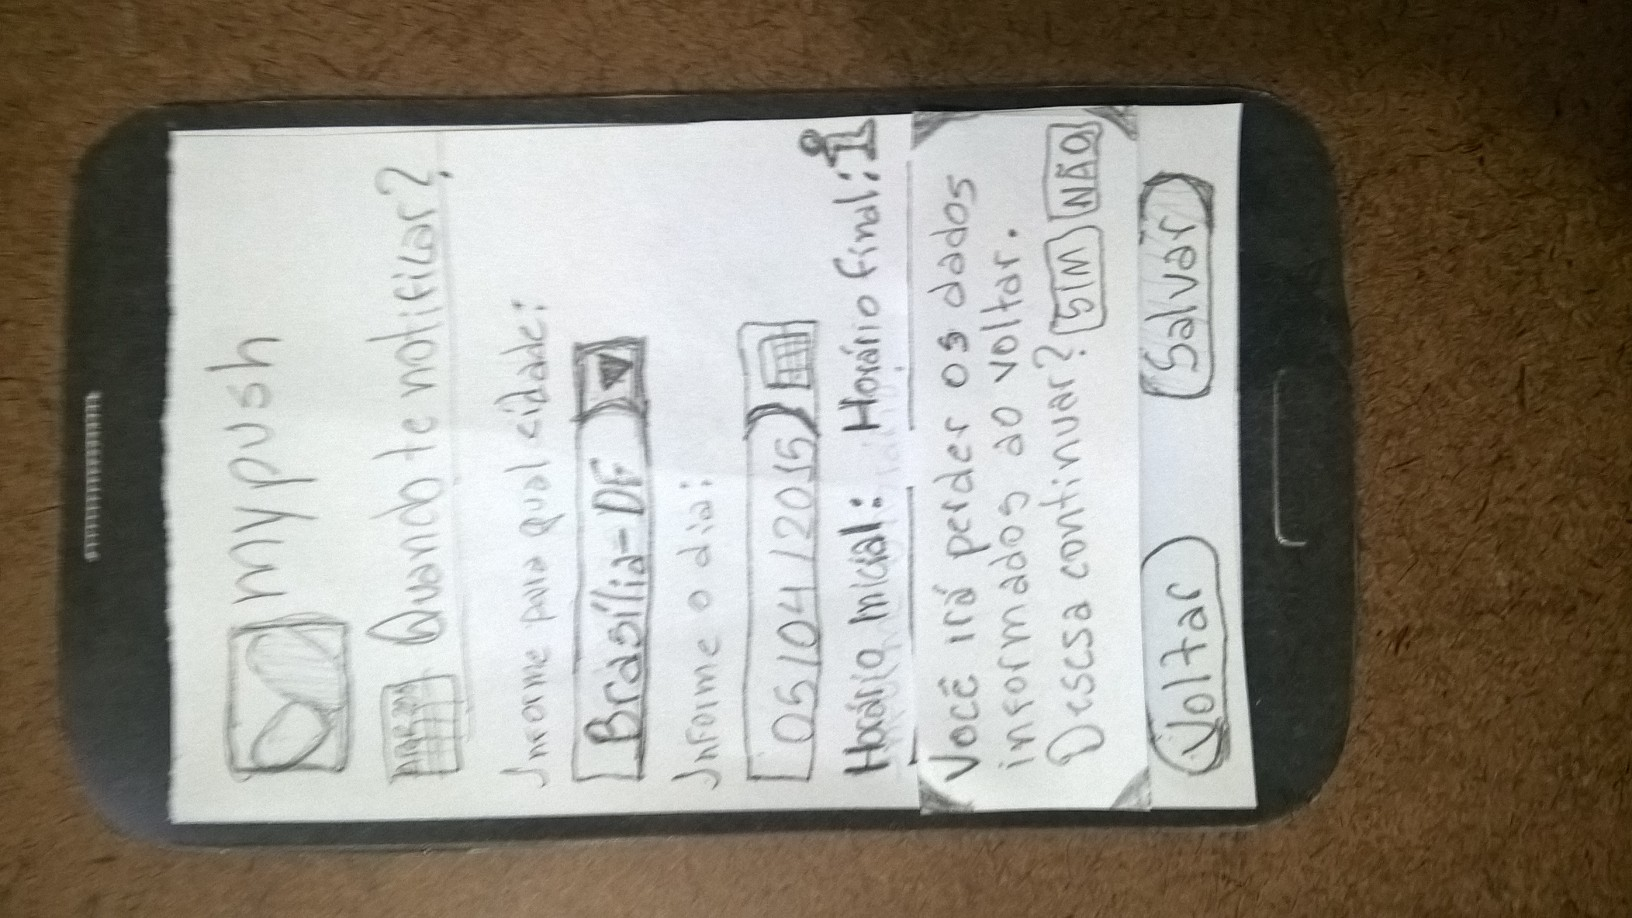
\includegraphics[scale=0.32, angle=-90]{editaveis/figuras/prototipo_papel_v2/confirmacao_perda_dados}
      \caption{Protótipo que ilustra a mensagem de confirmação para voltar para outra tela}
      \label{confirmacao_perda_dados_v2}
    \end{figure}
    
  \pagebreak
  \section*{Protótipo que ilustra a nova tela para editar uma notificação}

    \begin{figure}[!htbp]
      \centering
      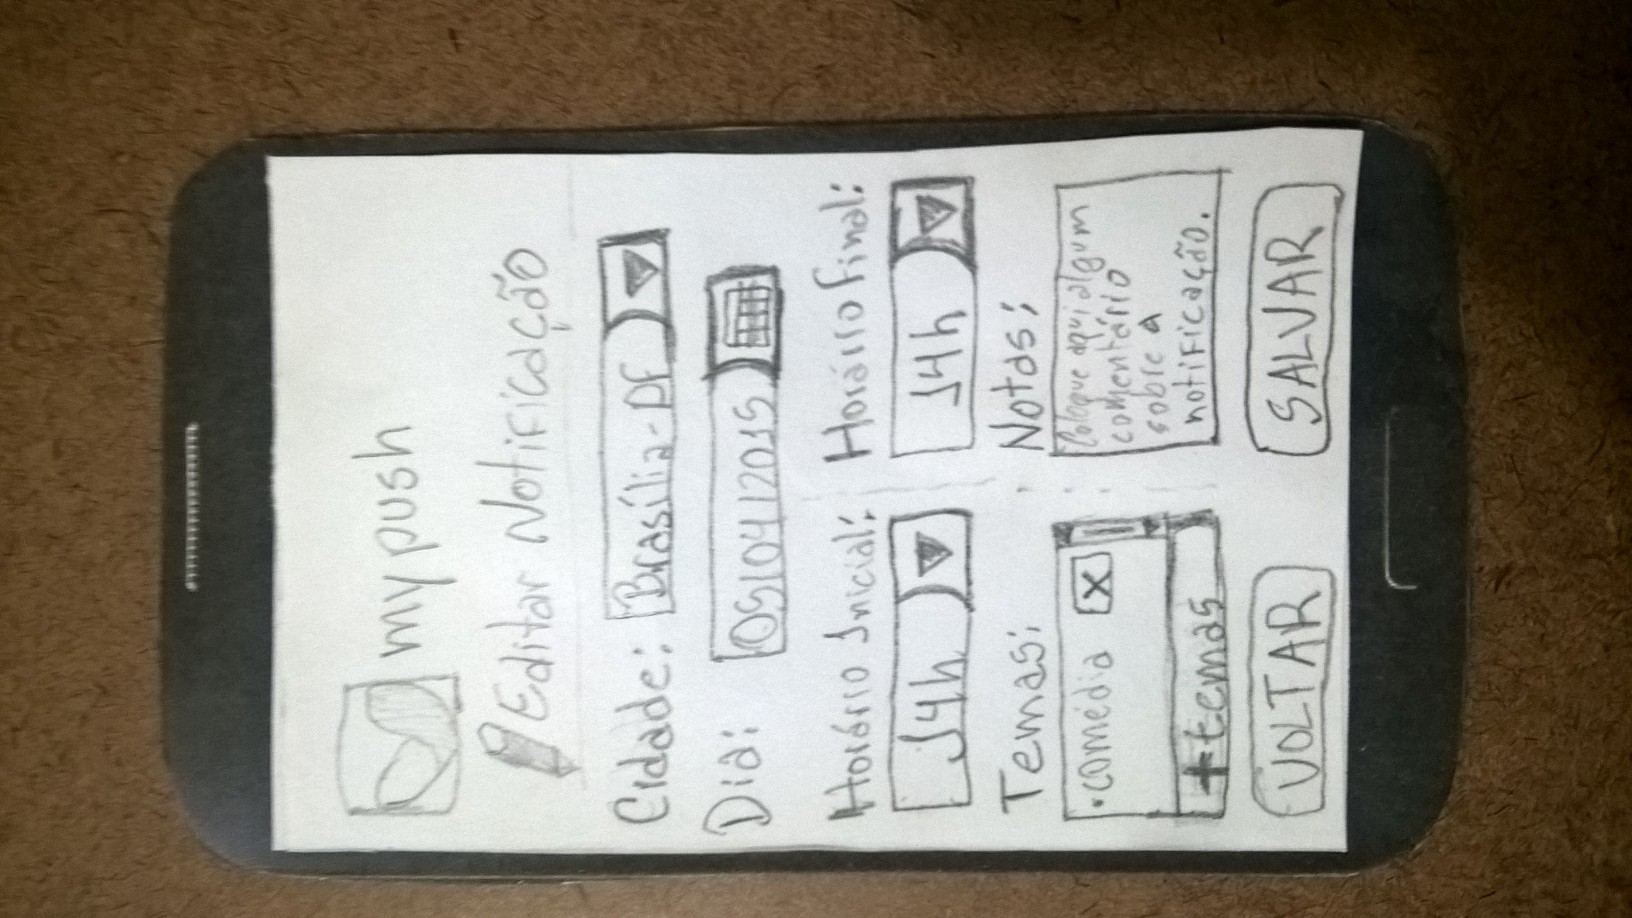
\includegraphics[scale=0.32, angle=-90]{editaveis/figuras/prototipo_papel_v2/editar_notificacao}
      \caption{Protótipo que ilustra a nova tela para editar uma notificação}
      \label{editar_notificacao_v2}
    \end{figure}
  
  \pagebreak
  \section*{Protótipo que ilustra a caixa para buscar mais temas}

    \begin{figure}[!htbp]
      \centering
      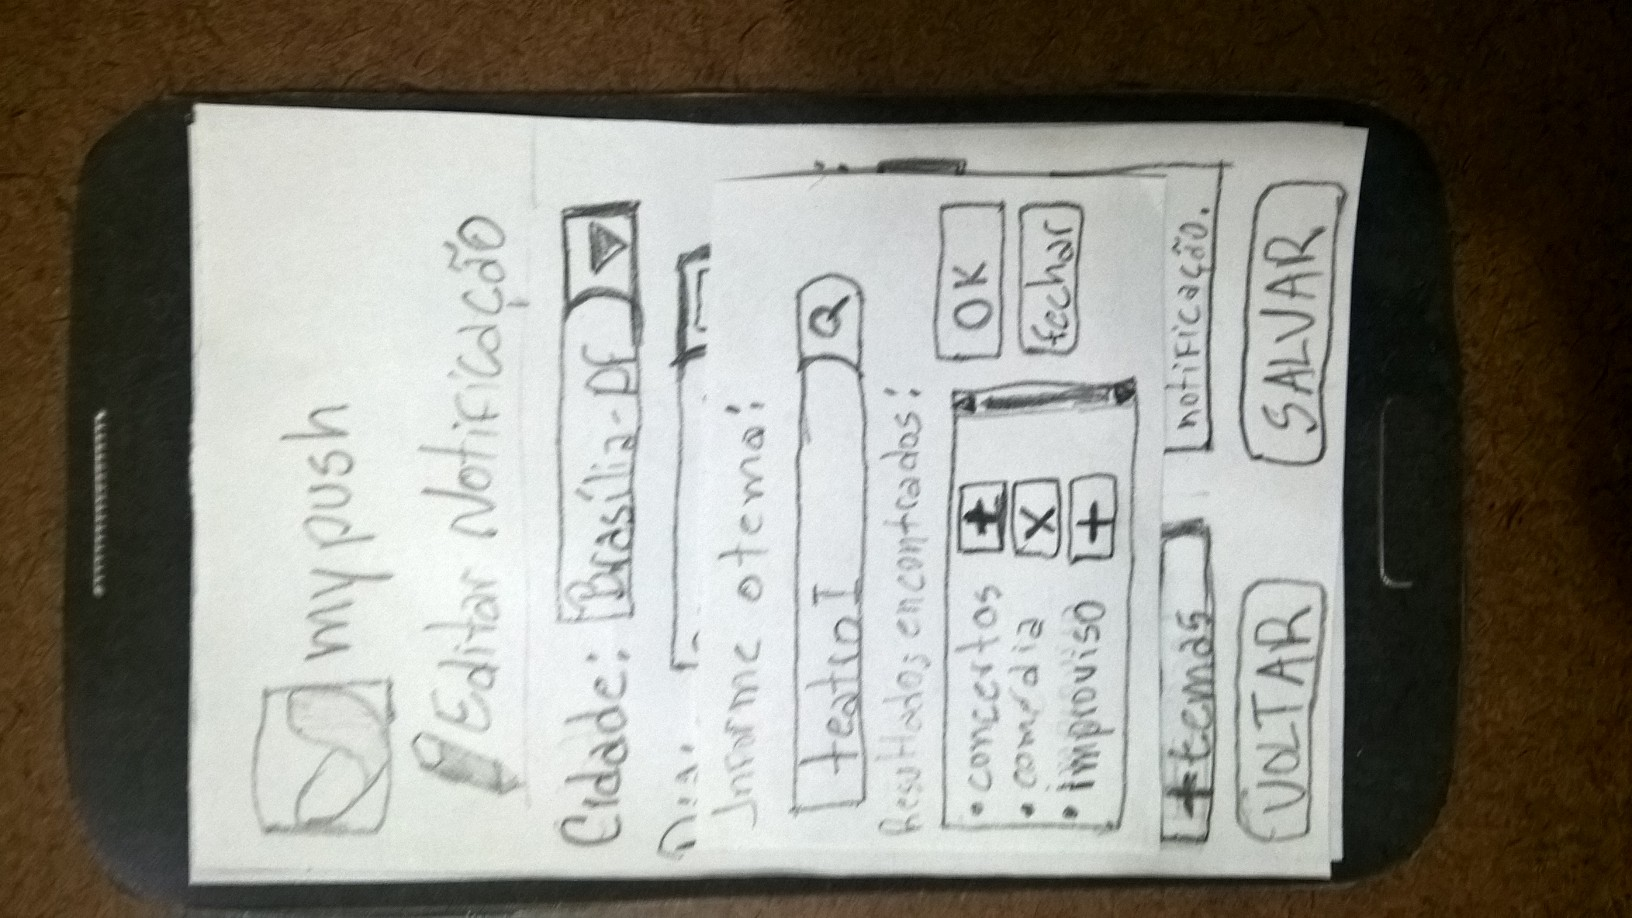
\includegraphics[scale=0.32, angle=-90]{editaveis/figuras/prototipo_papel_v2/editar_notificacao_mais_temas}
      \caption{Protótipo que ilustra a caixa para buscar mais temas}
      \label{editar_notificacao_mais_temas_v2}
    \end{figure}
  
  \pagebreak
  \section*{Protótipo que ilustra uma exclusão de uma notificação}

    \begin{figure}[!htbp]
      \centering
      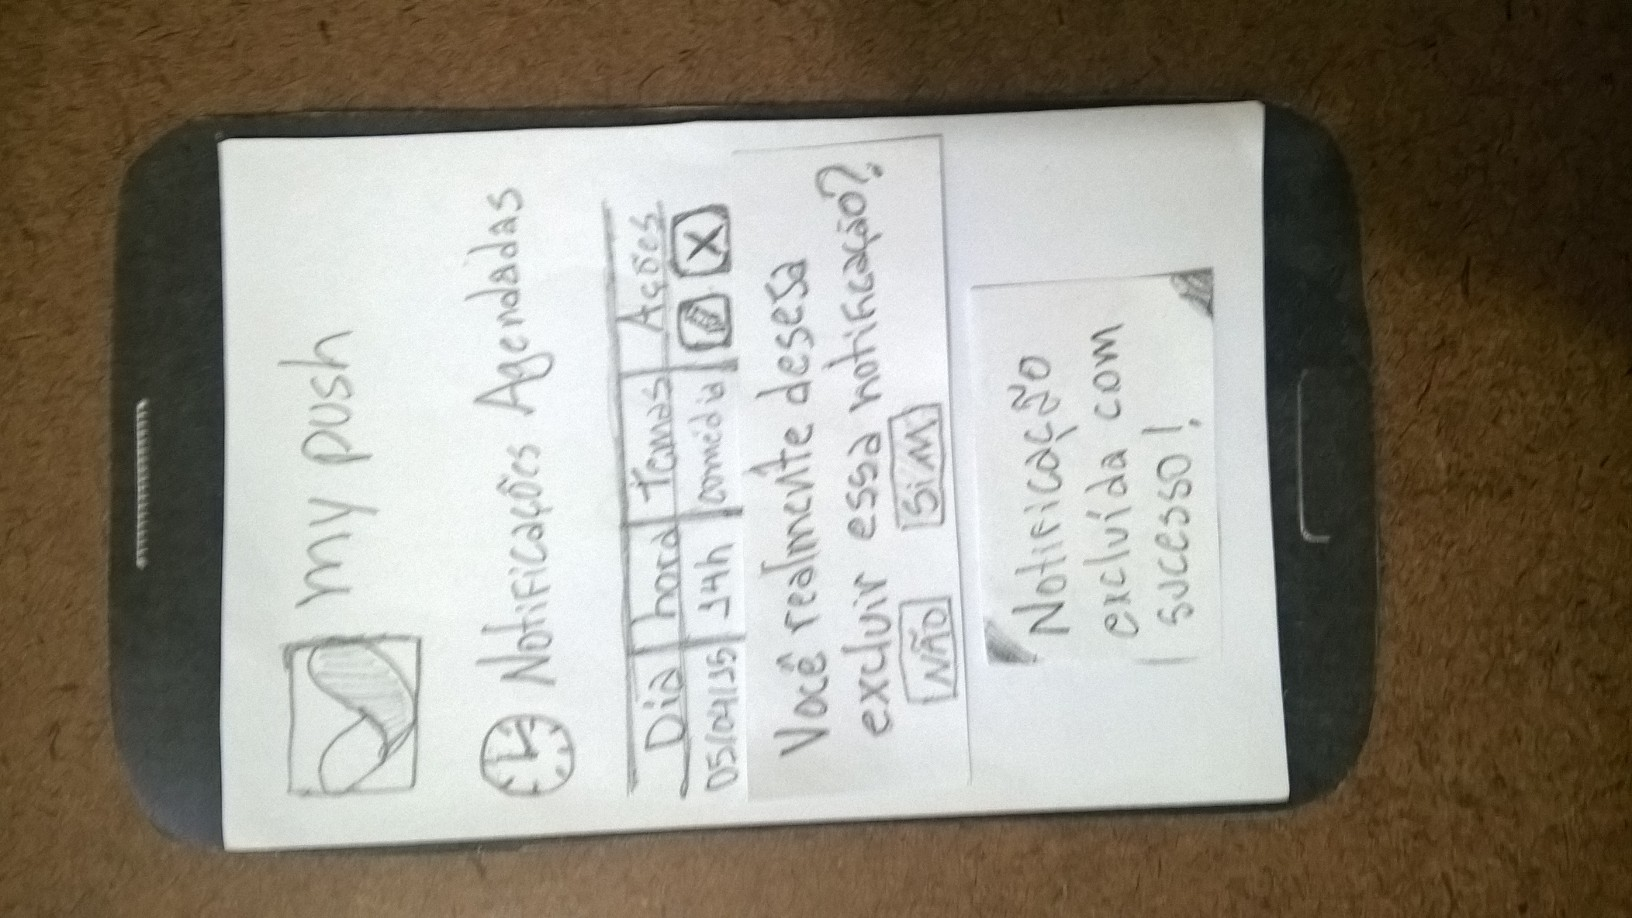
\includegraphics[scale=0.32, angle=-90]{editaveis/figuras/prototipo_papel_v2/confirmacao_exclusao_notificacao}
      \caption{Protótipo que ilustra uma exclusão de uma notificação}
      \label{confirmacao_exclusao_notificacao_v2}
    \end{figure}
  
  \pagebreak
  \section*{Protótipo que ilustra a página de notificações agendas sem notificações}

    \begin{figure}[!htbp]
      \centering
      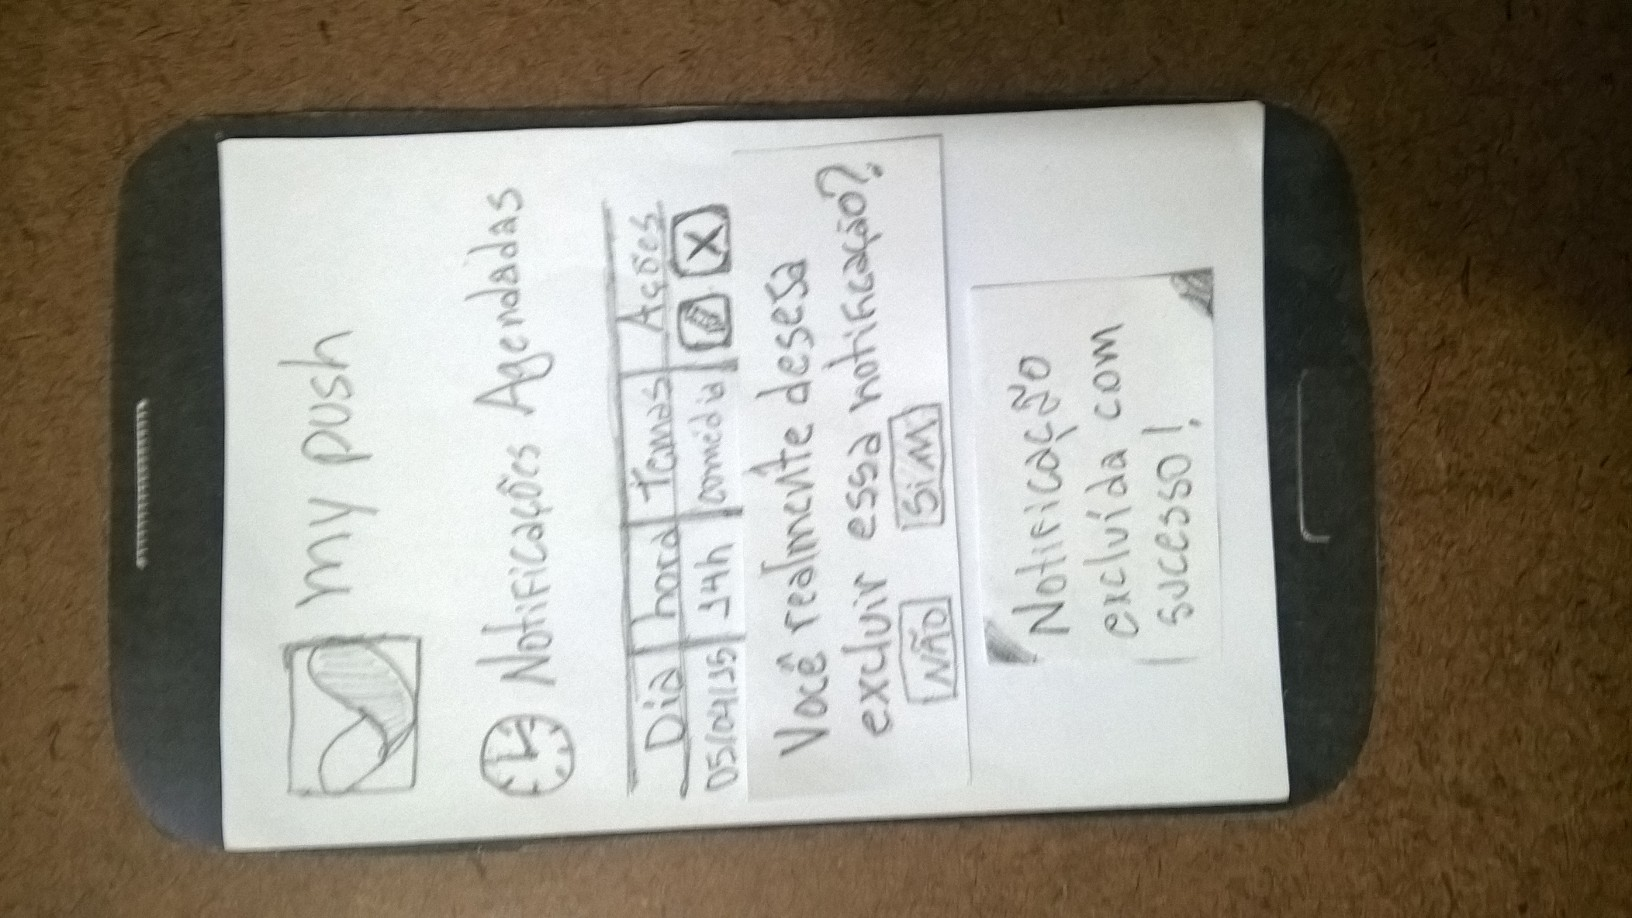
\includegraphics[scale=0.32, angle=-90]{editaveis/figuras/prototipo_papel_v2/confirmacao_exclusao_notificacao}
      \caption{Protótipo que ilustra a página de notificações agendas sem notificações (após a exclusão)}
      \label{confirmacao_exclusao_notificacao_v2}
    \end{figure}
    
\chapter{Protótipo de alta fidelidade - Versão 1.0}

  \section*{Protótipo que ilustra a página de próximas notificações}

    \begin{figure}[!htbp]
      \centering
      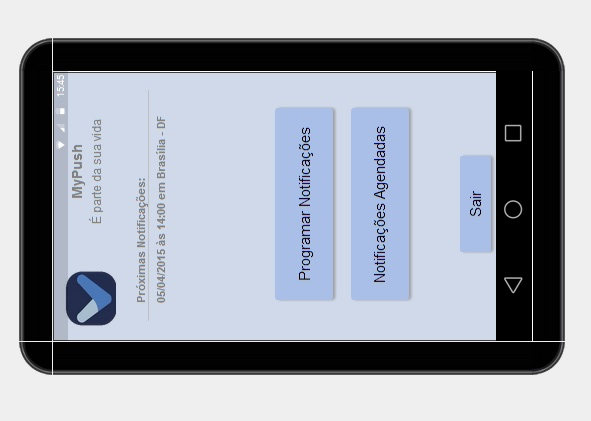
\includegraphics[scale=0.5, angle=-90]{editaveis/figuras/prototipo_alta_fidelidade_v1/1_1}
      \caption{Protótipo que ilustra a página de próximas notificações(versão 1.0)}
      \label{v1}
    \end{figure}
    
      \section*{Protótipo que ilustra a primeira página de programar notificações}

    \begin{figure}[!htbp]
      \centering
      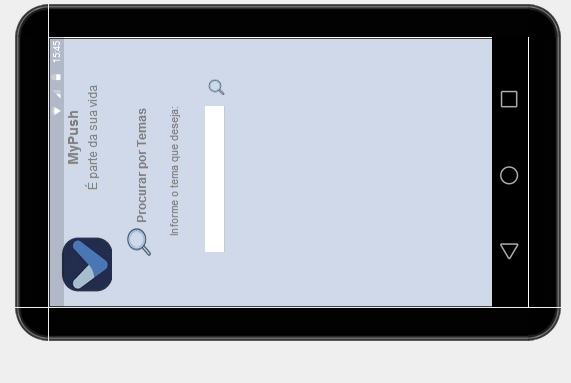
\includegraphics[scale=0.5, angle=-90]{editaveis/figuras/prototipo_alta_fidelidade_v1/1_2}
      \caption{Protótipo que ilustra a primeira página de programar notificações(versão 1.0)}
      \label{v1}
    \end{figure}
    
      \section*{Protótipo que ilustra a página de resultados encontrados}

    \begin{figure}[!htbp]
      \centering
      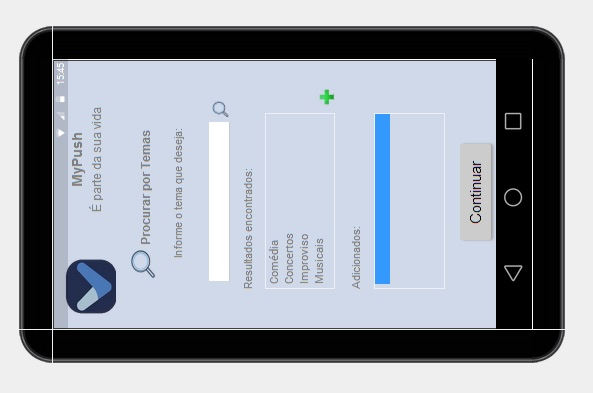
\includegraphics[scale=0.5, angle=-90]{editaveis/figuras/prototipo_alta_fidelidade_v1/1_3}
      \caption{Protótipo que ilustra a página de resultados encontrados(versão 1.0)}
      \label{v1}
    \end{figure}
    
      \section*{Protótipo que ilustra a página de tema adicionado}

    \begin{figure}[!htbp]
      \centering
      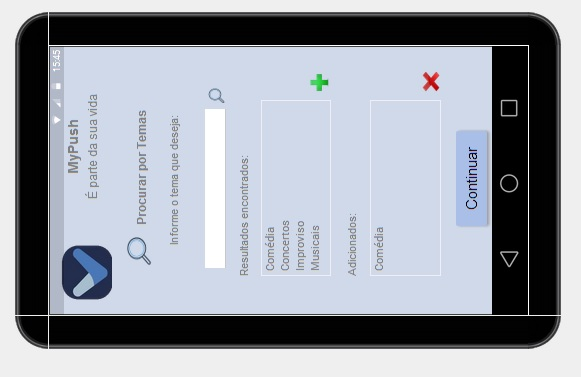
\includegraphics[scale=0.5, angle=-90]{editaveis/figuras/prototipo_alta_fidelidade_v1/1_4}
      \caption{Protótipo que ilustra a página de tema adicionado(versão 1.0)}
      \label{v1}
    \end{figure}
    
      \section*{Protótipo que ilustra a página de notificação salva}

    \begin{figure}[!htbp]
      \centering
      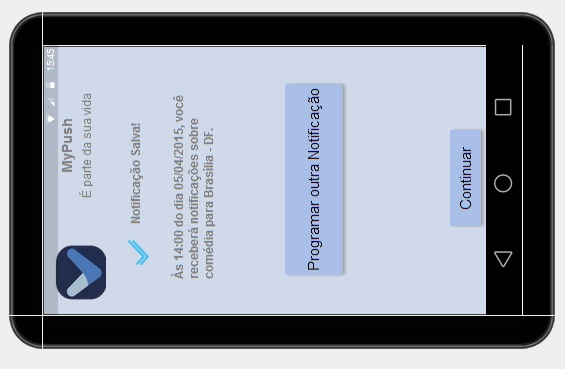
\includegraphics[scale=0.5, angle=-90]{editaveis/figuras/prototipo_alta_fidelidade_v1/1_5}
      \caption{Protótipo que ilustra a página de notificação salva(versão 1.0)}
      \label{v1}
    \end{figure}
    
      \section*{Protótipo que ilustra a página de cidades encontradas}

    \begin{figure}[!htbp]
      \centering
      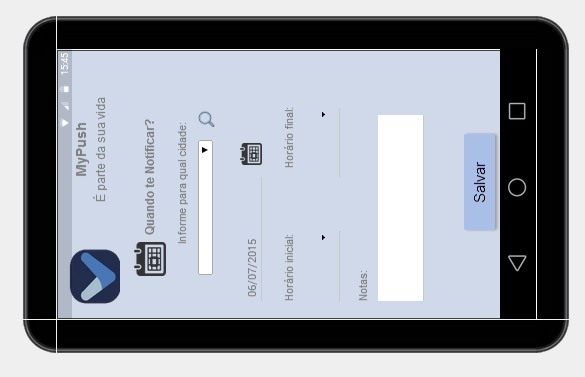
\includegraphics[scale=0.5, angle=-90]{editaveis/figuras/prototipo_alta_fidelidade_v1/1_6}
      \caption{Protótipo que ilustra a página de cidades encontradas(versão 1.0)}
      \label{v1}
    \end{figure}
    
      \section*{Protótipo que ilustra a página de notificações agendadas}

    \begin{figure}[!htbp]
      \centering
      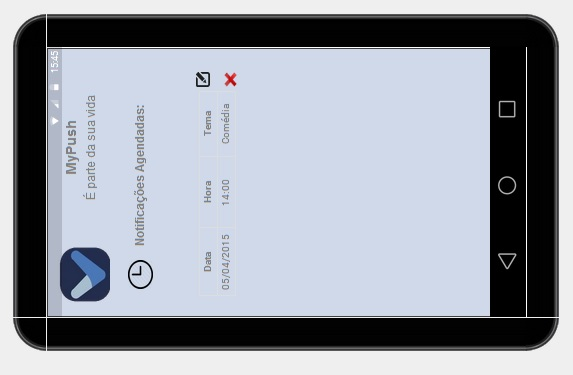
\includegraphics[scale=0.5, angle=-90]{editaveis/figuras/prototipo_alta_fidelidade_v1/1_7}
      \caption{Protótipo que ilustra a página de notificações agendadas(versão 1.0)}
      \label{v1}
    \end{figure}
    
      \section*{Protótipo que ilustra a página de editar notificações}

    \begin{figure}[!htbp]
      \centering
      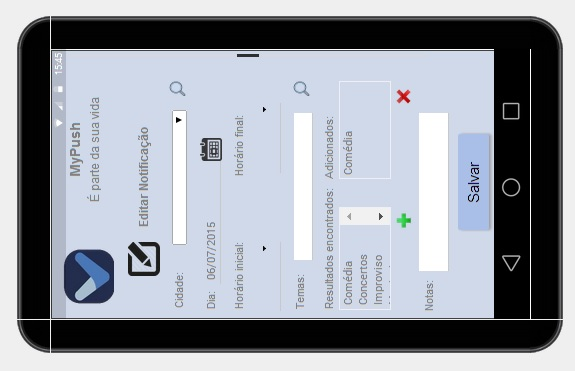
\includegraphics[scale=0.5, angle=-90]{editaveis/figuras/prototipo_alta_fidelidade_v1/1_8}
      \caption{Protótipo que ilustra a página de editar notificações(versão 1.0)}
      \label{v1}
    \end{figure}
    
      \section*{Protótipo que ilustra a página sem notificações agendadas}

    \begin{figure}[!htbp]
      \centering
      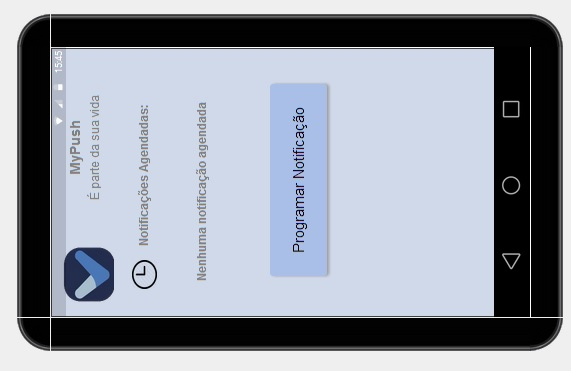
\includegraphics[scale=0.5, angle=-90]{editaveis/figuras/prototipo_alta_fidelidade_v1/1_9}
      \caption{Protótipo que ilustra a página sem notificações agendadas(versão 1.0)}
      \label{v1}
    \end{figure}
    
      \section*{Protótipo que ilustra a página que informa que seus dados serão perdidos}

    \begin{figure}[!htbp]
      \centering
      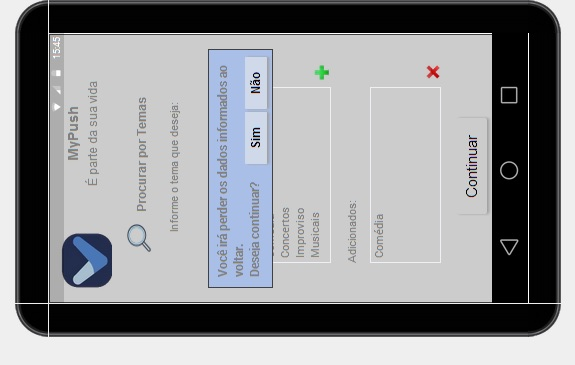
\includegraphics[scale=0.5, angle=-90]{editaveis/figuras/prototipo_alta_fidelidade_v1/1_10}
      \caption{Protótipo que ilustra a página que informa que seus dados serão perdidos(versão 1.0)}
      \label{v1}
    \end{figure}
    
      \section*{Protótipo que ilustra a página de confirmação da exlclusão}

    \begin{figure}[!htbp]
      \centering
      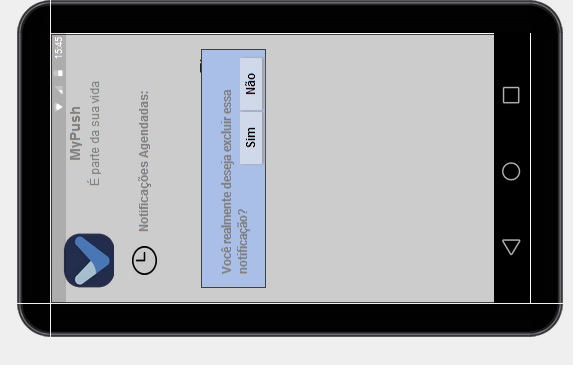
\includegraphics[scale=0.5, angle=-90]{editaveis/figuras/prototipo_alta_fidelidade_v1/1_11}
      \caption{Protótipo que ilustra a página de confirmação da exlclusão(versão 1.0)}
      \label{v1}
    \end{figure}
    
      \section*{Protótipo que ilustra a página de notificação excluida com sucesso}

    \begin{figure}[!htbp]
      \centering
      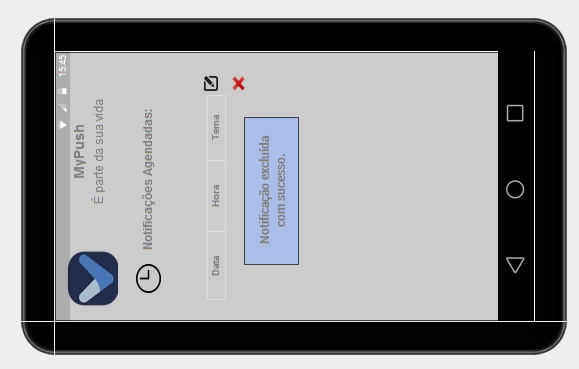
\includegraphics[scale=0.5, angle=-90]{editaveis/figuras/prototipo_alta_fidelidade_v1/1_12}
      \caption{Protótipo que ilustra a página de notificação excluida com sucesso(versão 1.0)}
      \label{v1}
    \end{figure}
    
      \section*{Protótipo que ilustra a página de informação sobre adicionar temas}

    \begin{figure}[!htbp]
      \centering
      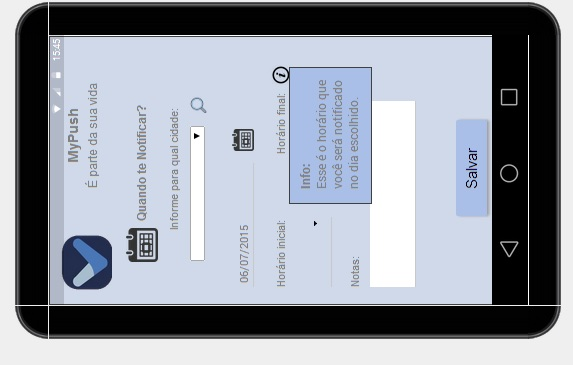
\includegraphics[scale=0.5, angle=-90]{editaveis/figuras/pprototipo_alta_fidelidade_v1/1_13}
      \caption{Protótipo que ilustra a página de informação sobre adicionar temas(versão 1.0)}
      \label{v1}
    \end{figure}
    
      \section*{Protótipo que ilustra a página editar notificações sem tema adicionado}

    \begin{figure}[!htbp]
      \centering
      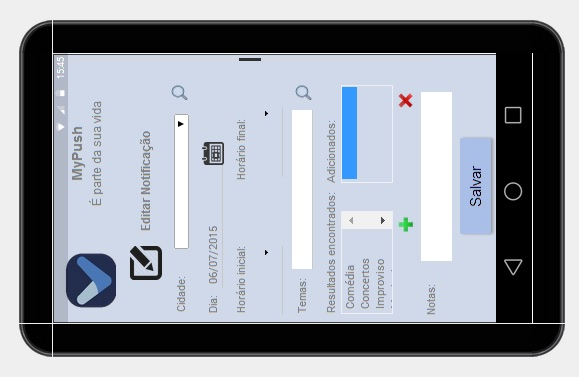
\includegraphics[scale=0.5, angle=-90]{editaveis/figuras/prototipo_alta_fidelidade_v1/1_14}
      \caption{Protótipo que ilustra a página editar notificações sem tema adicionado(versão 1.0)}
      \label{v1}
    \end{figure}
    
      \section*{Protótipo que ilustra a página de editado com sucesso}

    \begin{figure}[!htbp]
      \centering
      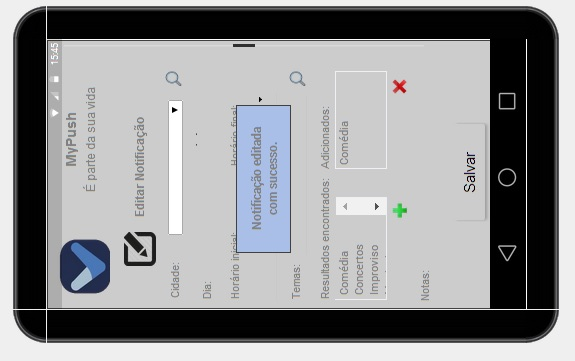
\includegraphics[scale=0.5, angle=-90]{editaveis/figuras/prototipo_alta_fidelidade_v1/1_15}
      \caption{Protótipo que ilustra a página de editado com sucesso(versão 1.0)}
      \label{v1}
    \end{figure}
    
      \section*{Protótipo que ilustra a página de início}

    \begin{figure}[!htbp]
      \centering
      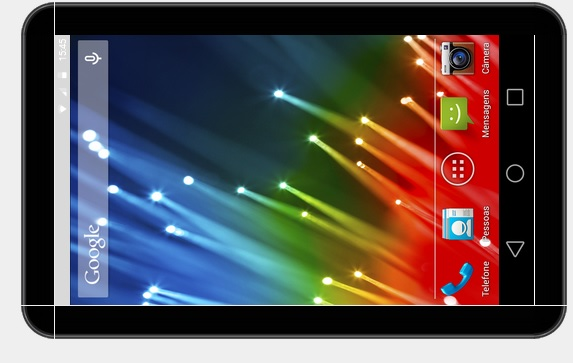
\includegraphics[scale=0.5, angle=-90]{editaveis/figuras/prototipo_alta_fidelidade_v1/1_16}
      \caption{Protótipo que ilustra a página de início(versão 1.0)}
      \label{v1}
    \end{figure}



\chapter{Protótipo de alta fidelidade - Versão 2.0}


    \section*{Protótipo que ilustra a página de próximas notificações}

    \begin{figure}[!htbp]
      \centering
      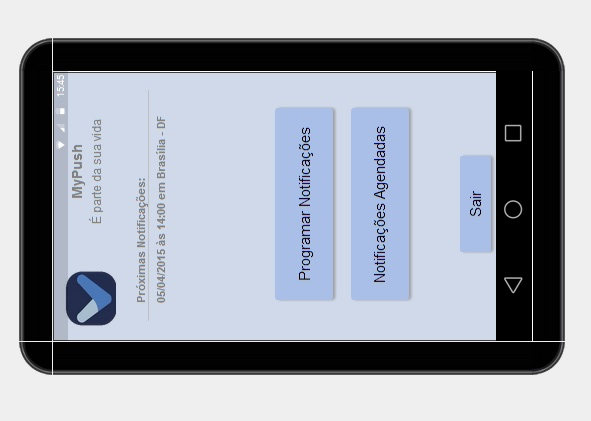
\includegraphics[scale=0.5, angle=-90]{editaveis/figuras/prototipo_alta_fidelidade_v2/2_1}
      \caption{Protótipo que ilustra a página de próximas notificações(versão 2.0)}
      \label{v2}
    \end{figure}
    
      \section*{Protótipo que ilustra a primeira página de programar notificações}

    \begin{figure}[!htbp]
      \centering
      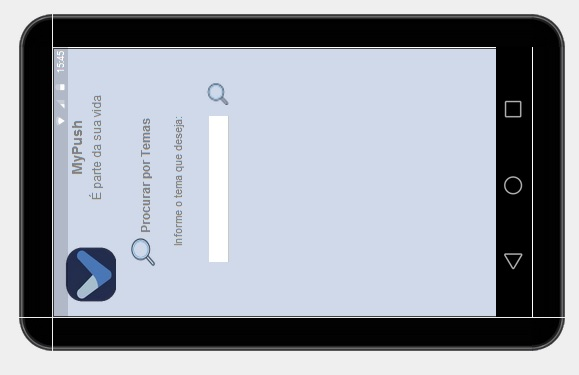
\includegraphics[scale=0.5, angle=-90]{editaveis/figuras/prototipo_alta_fidelidade_v2/2_2}
      \caption{Protótipo que ilustra a primeira página de programar notificações(versão 2.0)}
      \label{v2}
    \end{figure}
    
      \section*{Protótipo que ilustra a página de resultados encontrados}

    \begin{figure}[!htbp]
      \centering
      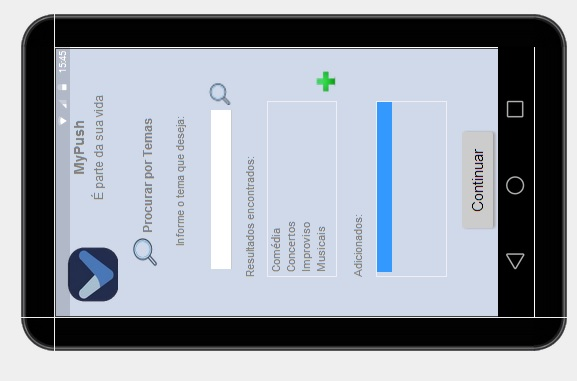
\includegraphics[scale=0.5, angle=-90]{editaveis/figuras/prototipo_alta_fidelidade_v2/2_3}
      \caption{Protótipo que ilustra a página de resultados encontrados(versão 2.0)}
      \label{v2}
    \end{figure}
    
      \section*{Protótipo que ilustra a página de tema adicionado}

    \begin{figure}[!htbp]
      \centering
      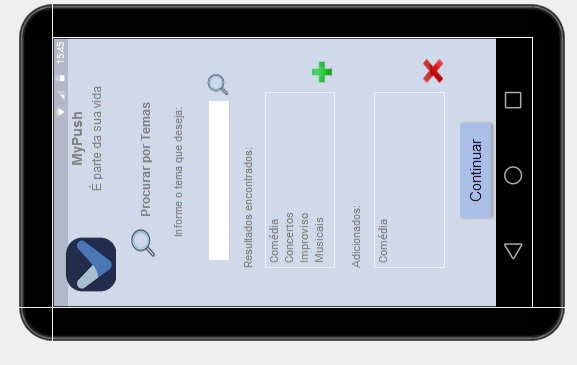
\includegraphics[scale=0.5, angle=-90]{editaveis/figuras/prototipo_alta_fidelidade_v2/2_4}
      \caption{Protótipo que ilustra a página de tema adicionado(versão 2.0)}
      \label{v2}
    \end{figure}
    
      \section*{Protótipo que ilustra a página de notificação salva}

    \begin{figure}[!htbp]
      \centering
      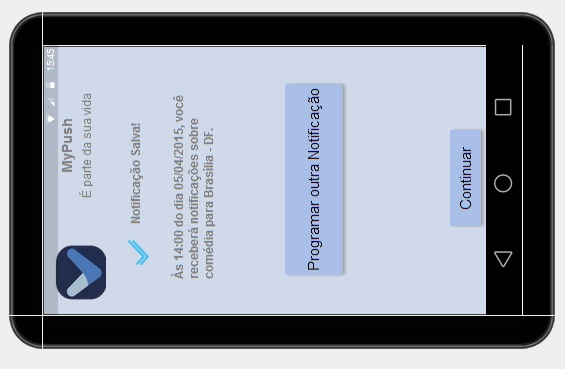
\includegraphics[scale=0.5, angle=-90]{editaveis/figuras/prototipo_alta_fidelidade_v2/2_5}
      \caption{Protótipo que ilustra a página de notificação salva(versão 2.0)}
      \label{v2}
    \end{figure}
    
      \section*{Protótipo que ilustra a página de cidades encontradas}

    \begin{figure}[!htbp]
      \centering
      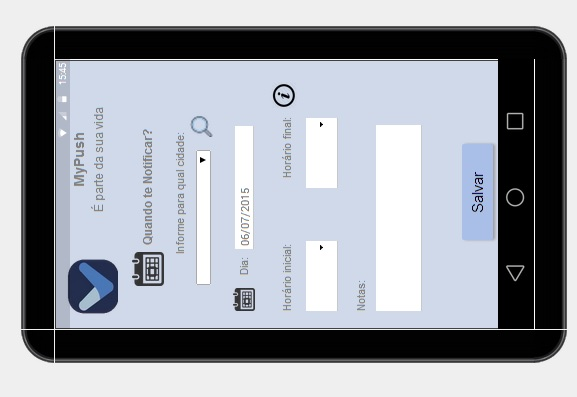
\includegraphics[scale=0.5, angle=-90]{editaveis/figuras/prototipo_alta_fidelidade_v2/2_6}
      \caption{Protótipo que ilustra a página de cidades encontradas(versão 2.0)}
      \label{v2}
    \end{figure}
    
      \section*{Protótipo que ilustra a página de notificações agendadas}

    \begin{figure}[!htbp]
      \centering
      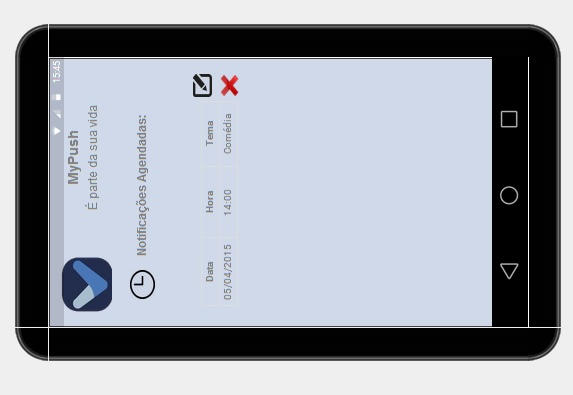
\includegraphics[scale=0.5, angle=-90]{editaveis/figuras/prototipo_alta_fidelidade_v2/2_7}
      \caption{Protótipo que ilustra a página de notificações agendadas(versão 2.0)}
      \label{v2}
    \end{figure}
    
      \section*{Protótipo que ilustra a página de editar notificações}

    \begin{figure}[!htbp]
      \centering
      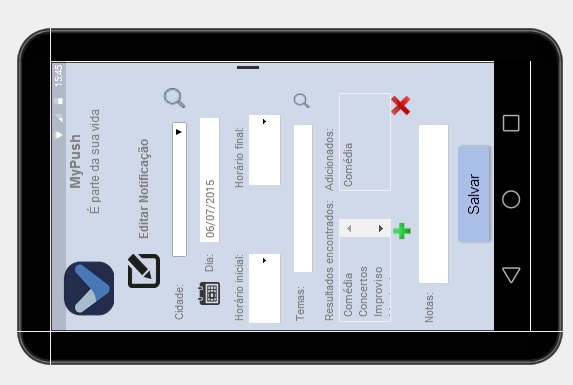
\includegraphics[scale=0.5, angle=-90]{editaveis/figuras/prototipo_alta_fidelidade_v2/2_8}
      \caption{Protótipo que ilustra a página de editar notificações(versão 2.0)}
      \label{v2}
    \end{figure}
    
      \section*{Protótipo que ilustra a página sem notificações agendadas}

    \begin{figure}[!htbp]
      \centering
      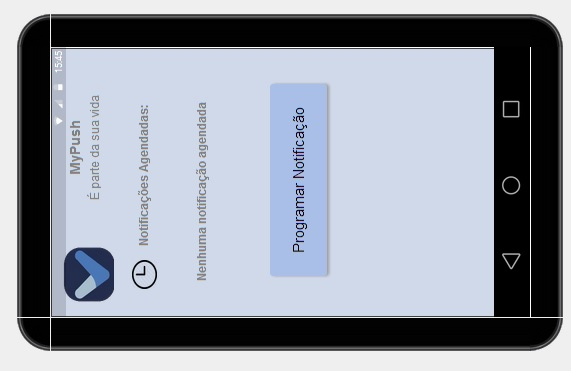
\includegraphics[scale=0.5, angle=-90]{editaveis/figuras/prototipo_alta_fidelidade_v2/2_9}
      \caption{Protótipo que ilustra a página sem notificações agendadas(versão 2.0)}
      \label{v2}
    \end{figure}
    
      \section*{Protótipo que ilustra a página que informa que seus dados serão perdidos}

    \begin{figure}[!htbp]
      \centering
      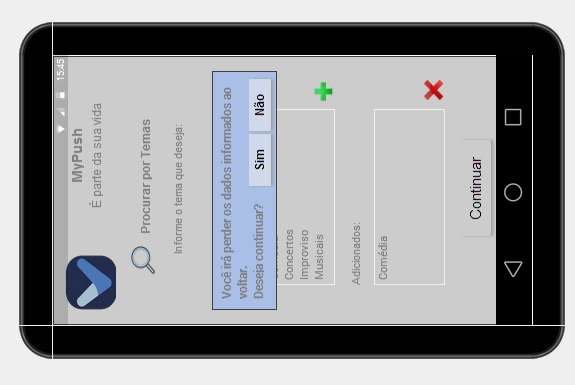
\includegraphics[scale=0.5, angle=-90]{editaveis/figuras/prototipo_alta_fidelidade_v2/2_10}
      \caption{Protótipo que ilustra a página que informa que seus dados serão perdidos(versão 2.0)}
      \label{v2}
    \end{figure}
    
      \section*{Protótipo que ilustra a página de confirmação da exlclusão}

    \begin{figure}[!htbp]
      \centering
      \includegraphics[scale=0.5, angle=-90]{editaveis/figuras/prototipo_alta_fidelidade_v2/2_11}
      \caption{Protótipo que ilustra a página de confirmação da exlclusão(versão 2.0)}
      \label{v2}
    \end{figure}
    
      \section*{Protótipo que ilustra a página de notificação excluida com sucesso}

    \begin{figure}[!htbp]
      \centering
      \includegraphics[scale=0.5, angle=-90]{editaveis/figuras/prototipo_alta_fidelidade_v2/2_12}
      \caption{Protótipo que ilustra a página de notificação excluida com sucesso(versão 2.0)}
      \label{v2}
    \end{figure}
    
      \section*{Protótipo que ilustra a página de informação sobre adicionar temas}

    \begin{figure}[!htbp]
      \centering
      \includegraphics[scale=0.5, angle=-90]{editaveis/figuras/pprototipo_alta_fidelidade_v2/2_13}
      \caption{Protótipo que ilustra a página de informação sobre adicionar temas(versão 2.0)}
      \label{v2}
    \end{figure}
    
      \section*{Protótipo que ilustra a página editar notificações sem tema adicionado}

    \begin{figure}[!htbp]
      \centering
      \includegraphics[scale=0.5, angle=-90]{editaveis/figuras/prototipo_alta_fidelidade_v2/2_14}
      \caption{Protótipo que ilustra a página editar notificações sem tema adicionado(versão 2.0)}
      \label{v2}
    \end{figure}
    
      \section*{Protótipo que ilustra a página de editado com sucesso}

    \begin{figure}[!htbp]
      \centering
      \includegraphics[scale=0.5, angle=-90]{editaveis/figuras/prototipo_alta_fidelidade_v2/2_15}
      \caption{Protótipo que ilustra a página de editado com sucesso(versão 2.0)}
      \label{v2}
    \end{figure}
    
      \section*{Protótipo que ilustra a página de início}

    \begin{figure}[!htbp]
      \centering
      \includegraphics[scale=0.5, angle=-90]{editaveis/figuras/prototipo_alta_fidelidade_v2/2_16}
      \caption{Protótipo que ilustra a página de início(versão 2.0)}
      \label{v2}
    \end{figure}


\chapter{Protótipo de alta fidelidade - Versão 3.0} 

    \section*{Protótipo que ilustra a página de próximas notificações}

    \begin{figure}[!htbp]
      \centering
      \includegraphics[scale=0.5, angle=-90]{editaveis/figuras/prototipo_alta_fidelidade_v3/3_1}
      \caption{Protótipo que ilustra a página de próximas notificações(versão 3.0)}
      \label{v3}
    \end{figure}
    
      \section*{Protótipo que ilustra a primeira página de programar notificações}

    \begin{figure}[!htbp]
      \centering
      \includegraphics[scale=0.5, angle=-90]{editaveis/figuras/prototipo_alta_fidelidade_v3/3_2}
      \caption{Protótipo que ilustra a primeira página de programar notificações(versão 3.0)}
      \label{v3}
    \end{figure}
    
      \section*{Protótipo que ilustra a página de resultados encontrados}

    \begin{figure}[!htbp]
      \centering
      \includegraphics[scale=0.5, angle=-90]{editaveis/figuras/prototipo_alta_fidelidade_v3/3_3}
      \caption{Protótipo que ilustra a página de resultados encontrados(versão 3.0)}
      \label{v3}
    \end{figure}
    
      \section*{Protótipo que ilustra a página de tema adicionado}

    \begin{figure}[!htbp]
      \centering
      \includegraphics[scale=0.5, angle=-90]{editaveis/figuras/prototipo_alta_fidelidade_v3/3_4}
      \caption{Protótipo que ilustra a página de tema adicionado(versão 3.0)}
      \label{v3}
    \end{figure}
    
      \section*{Protótipo que ilustra a página de notificação salva}

    \begin{figure}[!htbp]
      \centering
      \includegraphics[scale=0.5, angle=-90]{editaveis/figuras/prototipo_alta_fidelidade_v3/3_5}
      \caption{Protótipo que ilustra a página de notificação salva(versão 3.0)}
      \label{v3}
    \end{figure}
    
      \section*{Protótipo que ilustra a página de cidades encontradas}

    \begin{figure}[!htbp]
      \centering
      \includegraphics[scale=0.5, angle=-90]{editaveis/figuras/prototipo_alta_fidelidade_v3/3_6}
      \caption{Protótipo que ilustra a página de cidades encontradas(versão 3.0)}
      \label{v3}
    \end{figure}
    
      \section*{Protótipo que ilustra a página de notificações agendadas}

    \begin{figure}[!htbp]
      \centering
      \includegraphics[scale=0.5, angle=-90]{editaveis/figuras/prototipo_alta_fidelidade_v3/3_7}
      \caption{Protótipo que ilustra a página de notificações agendadas(versão 3.0)}
      \label{v3}
    \end{figure}
    
      \section*{Protótipo que ilustra a página de editar notificações}

    \begin{figure}[!htbp]
      \centering
      \includegraphics[scale=0.5, angle=-90]{editaveis/figuras/prototipo_alta_fidelidade_v3/3_8}
      \caption{Protótipo que ilustra a página de editar notificações(versão 3.0)}
      \label{v3}
    \end{figure}
    
      \section*{Protótipo que ilustra a página sem notificações agendadas}

    \begin{figure}[!htbp]
      \centering
      \includegraphics[scale=0.5, angle=-90]{editaveis/figuras/prototipo_alta_fidelidade_v3/3_9}
      \caption{Protótipo que ilustra a página sem notificações agendadas(versão 3.0)}
      \label{v3}
    \end{figure}
    
      \section*{Protótipo que ilustra a página que informa que seus dados serão perdidos}

    \begin{figure}[!htbp]
      \centering
      \includegraphics[scale=0.5, angle=-90]{editaveis/figuras/prototipo_alta_fidelidade_v3/3_10}
      \caption{Protótipo que ilustra a página que informa que seus dados serão perdidos(versão 3.0)}
      \label{v3}
    \end{figure}
    
      \section*{Protótipo que ilustra a página de confirmação da exlclusão}

    \begin{figure}[!htbp]
      \centering
      \includegraphics[scale=0.5, angle=-90]{editaveis/figuras/prototipo_alta_fidelidade_v3/3_11}
      \caption{Protótipo que ilustra a página de confirmação da exlclusão(versão 3.0)}
      \label{v3}
    \end{figure}
    
      \section*{Protótipo que ilustra a página de notificação excluida com sucesso}

    \begin{figure}[!htbp]
      \centering
      \includegraphics[scale=0.5, angle=-90]{editaveis/figuras/prototipo_alta_fidelidade_v3/3_12}
      \caption{Protótipo que ilustra a página de notificação excluida com sucesso(versão 3.0)}
      \label{v3}
    \end{figure}
    
      \section*{Protótipo que ilustra a página de informação sobre adicionar temas}

    \begin{figure}[!htbp]
      \centering
      \includegraphics[scale=0.5, angle=-90]{editaveis/figuras/pprototipo_alta_fidelidade_v3/3_13}
      \caption{Protótipo que ilustra a página de informação sobre adicionar temas(versão 3.0)}
      \label{v3}
    \end{figure}
    
      \section*{Protótipo que ilustra a página editar notificações sem tema adicionado}

    \begin{figure}[!htbp]
      \centering
      \includegraphics[scale=0.5, angle=-90]{editaveis/figuras/prototipo_alta_fidelidade_v3/3_14}
      \caption{Protótipo que ilustra a página editar notificações sem tema adicionado(versão 3.0)}
      \label{v3}
    \end{figure}
    
      \section*{Protótipo que ilustra a página de editado com sucesso}

    \begin{figure}[!htbp]
      \centering
      \includegraphics[scale=0.5, angle=-90]{editaveis/figuras/prototipo_alta_fidelidade_v3/3_15}
      \caption{Protótipo que ilustra a página de editado com sucesso(versão 3.0)}
      \label{v3}
    \end{figure}
    
      \section*{Protótipo que ilustra a página de início}

    \begin{figure}[!htbp]
      \centering
      \includegraphics[scale=0.5, angle=-90]{editaveis/figuras/prototipo_alta_fidelidade_v3/3_16}
      \caption{Protótipo que ilustra a página de início(versão 3.0)}
      \label{v3}
    \end{figure}

\end{apendicesenv}
